\documentclass{beamer}

\usefonttheme[onlymath]{serif}
\usepackage[utf8]{inputenc}
\usepackage{amsmath}
\usepackage{array}
\usepackage{graphicx}
\usepackage{mathtools}
\usepackage{minted}
\usepackage{hyperref}
\hypersetup{
    colorlinks=true,
    linkcolor=blue,
}
\usemintedstyle{manni}
\newminted{python}{fontsize=\footnotesize}
\newminted{cython}{fontsize=\footnotesize}

\usetheme{Pittsburgh}
% \beamertemplatenavigationsymbolsempty

\usepackage{tikz,tkz-euclide}
\usetikzlibrary{angles}
\usetikzlibrary{decorations.markings}
\usetikzlibrary{arrows.meta}
\tikzset{%
  ->-/.style={decoration={markings, mark=at position 0.5 with {\arrow{>}}},
              postaction={decorate}},
  ->>-/.style={decoration={markings, mark=at position 0.5 with {\arrow{>>}}},
               postaction={decorate}},
  -|-/.style={decoration={markings, mark=at position 0.5 with {|}},
              postaction={decorate}},
}

\newtheoremstyle{case}{}{}{}{}{}{:}{ }{}
\theoremstyle{case}
\newtheorem{case}{Case}

\usepackage{pgfpages}
\setbeamertemplate{note page}{\pagecolor{yellow!5}\insertnote}
\setbeameroption{show notes on second screen=right}

\DeclareMathOperator{\md}{Manhattan Distance}
\DeclareMathOperator{\BigO}{O}

\title{Crunching Numbers with NumPy and Cython}
\author{Brian Lester}
\institute{Interactions}
\date{January 2, 2019}

\begin{document}

\def\R{\mathbb{R}}
\frame{\titlepage}

\begin{section}{Bio}

\begin{frame}
    \frametitle{Me}
    \begin{itemize}
        \item Work on NLP at Interactions specializing in Deep Learning
        \item Published/Maintain several python packages
        \begin{itemize}
            \item \href{https://github.com/blester125/string-distance}{string-distance}
            \item \href{https://github.com/blester125/text-rank}{text-rank}
            \item \href{https://github.com/dpressel/mead-baseline}{mead-baseline}
        \end{itemize}
    \end{itemize}
    \note{
        \begin{itemize}
            \item We use chat bots to ``facilitate customer care interaction'' aka to build better chat bots
            \item I mostly do DL and am a big Nerd so if you every want to talk about ML for NLP I'm game
            \item Python is my daily driver
            \item Have several packages on PyPI including ones written in cython (string-distance), the subject of today's talk
        \end{itemize}
    }
\end{frame}

\end{section} %Bio

\begin{section}{Background}

\begin{frame}
    \frametitle{The Problem}
    \begin{center}
    \begin{figure}
        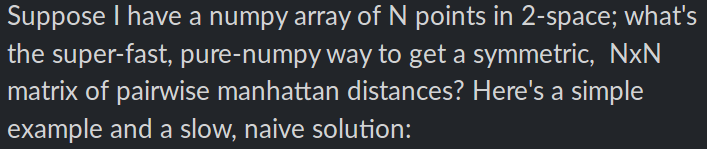
\includegraphics[width=\textwidth]{images/problem.png}
        \caption{\href{https://a2mads.herokuapp.com/}{Ann Arbor Machine Learning and Data Science Slack}}
    \end{figure}
    \end{center}
    \note{
        \begin{itemize}
            \item a2mads is the Ann Arbor Machine Learning and Data Science Slack
            \item There aren't a lot of messages flying about but when someone asks a question there is normally a lot if discussion
            \item This user was asking that given a list of points what is the distance between a point and every other point in the list for each item in the list
            \item There was a long thread about how to optimize his solution, we will walk through some of them.
        \end{itemize}
    }
\end{frame}

\begin{subsection}{Manhattan Distance}

\begin{frame}<1>[label=md]
    \frametitle{Manhattan Distance}
    \begin{itemize}
        \item<1-> The distance between points measured along axes at right angles
        \item<2-> Also called the L1, cityblock, or taxi distance
    \end{itemize}
    \note{
        \begin{itemize}
            \item Distance if you can only move along the axes
            \item Contrast with euclidean distance where we can move diagonally and go straight there.
            \item Like you have directions to somewhere in manhattan, you can't smash through a building, you need to drive along the streets
        \end{itemize}
    }
\end{frame}

\begin{frame}<1>[label=block]
    \begin{center}
        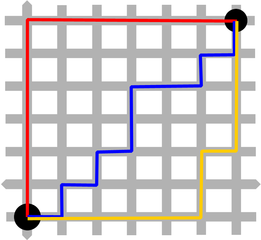
\includegraphics[width=0.9\textwidth]{images/manhattan.png}
    \end{center}
    \note<1>{
        \begin{itemize}
            \item Here we can see example of moving between points as the Manhattan distance does
        \end{itemize}
    }
    \note<2>{
        \begin{itemize}
            \item As suggested by the calculation for Manhattan Distance all of these paths have the same length, the next few slides sketch out why these are all the same but that isn't very important to us
            \item Point out the absolute distance between point dims on the red line, $6$ up $6$ over for a distance of $12$
            \item All paths are length $12$
        \end{itemize}
    }
\end{frame}

\againframe<2->{md}

\begin{frame}
    \frametitle{Manhattan Distance}
        A point with $M$ dimensions is a vector of $M$ numbers where the values at index $i$ is the distance along the $i^{th}$ axis.
        \begin{align*}
            X &\in \R^{M} \\
            Y &\in \R^{M} \\
            \md(X, Y) &= \sum_i^M | X_i - Y_i |
        \end{align*}
        \note{
            \begin{itemize}
                \item While the Manhattan distance works for real numbers we will only be looking at Ints in code
            \end{itemize}
        }
\end{frame}

\againframe<2>{block}

\begin{frame}
    \frametitle{Proof of Equal Lengths}
    \begin{columns}
        \column{0.5\textwidth}
          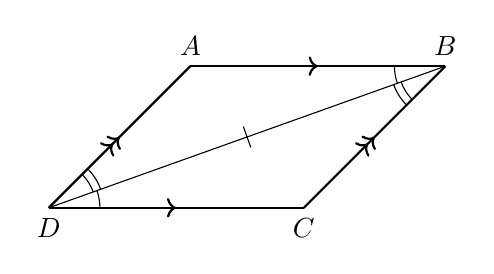
\begin{tikzpicture}[xslant=1,xscale=1.8,scale=1.8]
              \coordinate (D) at (0,0);
              \coordinate (A) at (0,1);
              \coordinate (B) at (1,1);
              \coordinate (C) at (1,0);
              \draw[-,thick,->-] (A) node[above]{$A$} -- (B) node[above]{$B$};
              \draw[-,thick,->-] (D) node[below]{$D$} -- (C) node[below]{$C$};
              \draw[-,thick,->>-] (D) -- (A);
              \draw[-,thick,->>-] (C) -- (B);
              \draw[-] (D) -- (B);
              \tkzMarkSegment[mark=|](D,B)
              \draw pic[draw=black,-,angle eccentricity=1.2,angle radius=0.6cm] {angle=B--D--A};
              \draw pic[draw=black,-,angle eccentricity=1.2,angle radius=0.7cm] {angle=B--D--A};
              \draw pic[draw=black,-,angle eccentricity=1.2,angle radius=0.6cm] {angle=D--B--C};
              \draw pic[draw=black,-,angle eccentricity=1.2,angle radius=0.7cm] {angle=D--B--C};
              \draw pic[draw=black,-,angle eccentricity=1.2,angle radius=0.65cm] {angle=A--B--D};
              \draw pic[draw=black,-,angle eccentricity=1.2,angle radius=0.65cm] {angle=C--D--B};
          \end{tikzpicture}
        \column{0.5\textwidth}
            \begin{proof}
            let $\overline{AB} \parallel \overline{DC}$ and $\overline{AD} \parallel \overline{BC}$ by the definition of a parallelogram.
            \begin{align*}
                \angle ABD &\cong \angle CDB \\
                \angle ADB &\cong \angle CBD \\
                \overline{DB} &= \overline{DB} \\
                \triangle ADB &\cong \triangle{CBD} \\
                \overline{AB} &= \overline{DC} \\
                \overline{AD} &= \overline{BC}
            \end{align*}
            \end{proof}
    \end{columns}
    \note{
        \begin{itemize}
            \item Quick overview of how on a regular grid you can move around a block in either direction and it will be the same length.
            \item DB is a transversal of both sets of parallel lines
            \item ABD and CDB are congruent because they are alternate interior angles
            \item ADB and DBC are congruent because they are alternate interior angles
            \item It is the same length as itself
            \item Triangles are congruent by angle side angle
            \item AB and CD are the same because they are the same sides of congruent triangles
            \item AD and CB are the same because they are the same sides of congruent triangles
        \end{itemize}
    }
\end{frame}

\begin{frame}
    \frametitle{All Paths Equal}
    \begin{itemize}
        \item Let $R$ be a move $1$ step \textit{right} and $U$ be a move $1$ step \textit{up}. \\
        \item Let the source point be $(0, 0)$ in our new coordinate system and the target be $(p, q)$. \\
        \item Any possible path from source to target will have $p$ $R$ moves and $q$ $U$ moves. \\
        \item There are $p + q$ moves in total. \\
        \item There are $\begin{pmatrix}
                p + q \\
                p
              \end{pmatrix}$ possible paths all of the same length
        \item If you make an extra $R$ or $U$ move you will not be at your target and will need to make extra steps so it will not be the shortest path.
    \end{itemize}
    \note{
        \begin{itemize}
            \item This is a quick overview on why all paths between two points have the same length
            \item You can scramble the order of moves and the path still has the same number of $R$s and $U$s but ends at the same spot
            \item It also sketches why the path length is always the length + height of the rectangle we make with the points as boxes
            \item This matches the formula where we take the absolute difference between points and sum across dimensions
            \item you can have a more rigorous proof via induction / contradiction that is based on the fact that if there was any shorter way to get to the next point then we could have gotten to this point through that but I didn't write it out here.
            \item The basic point is that because all paths are equal we can just look at the differences between the start and end, we don't need to care about the path take there.
        \end{itemize}
    }
\end{frame}

\end{subsection} %Manhattan Distance

\begin{frame}
    \frametitle{NumPy}
    \begin{itemize}
        \item<1-> \href{https://docs.scipy.org/doc/numpy/reference/}{NumPy}: A collection of linear algebra functions that operate on a \texttt{ndarray}
        \item<2-> \texttt{ndarray} is a typed container that can represent multi-dimensional arrays
        \item<3-> The majority of functionality is implemented in C extensions for speed
    \end{itemize}
    \note{
        \begin{itemize}
            \item \texttt{ndarray} has a data type
            \begin{itemize}
                \item all the items in it need to be the same and they can be stored contiguously in memory.
                \item So instead of following pointers for to the object for each element in a python list we can access the element directly
                \item This makes access fast and because they are together in memory we get better cache utilization
            \end{itemize}
            \item \texttt{ndarray} is a multi dimensional array
            \begin{itemize}
                \item a thing is a scalar
                \item a list of things is an array (or vector)
                \item a list of arrays is a matrix
                \item a list of matrices is a \texttt{ndarray}
                \item You can index like \texttt{x[i, j, k]}
                \item can have an arbitrary dimensions
            \end{itemize}
            \item A C extension is code written in C that can be called from python. You can use the speed of C and let go of the GIL. Loses ease of Python
        \end{itemize}
    }
\end{frame}

\begin{frame}
    \frametitle{Cython}
    \begin{itemize}
        \item<1-> \href{https://cython.org/}{Cython} is a compiler for Python and Cython
        \item<2-> Cython is also a language that looks more like python than C, but adds types
        \item<3-> It creates C extensions
        \item<4-> It can compile pure python code
        \item<5-> You can call python code from inside the cython code (and therefore from inside the C extension)
        \item<6-> Makes it easy to wrap C libraries
        \item<7-> Some large libraries like \href{https://spacy.io/}{SpaCy} are all cython
        \item<8-> \texttt{pip install cython}
    \end{itemize}
    \note{
        \begin{itemize}
            \item Cython is a superset of python, adds things like static types
            \item Compiling just python gives a slight speed boost
            \item You can also write code that releases the GIL so multithreading is possible
            \item We will see an example of why calling python code is nice
        \end{itemize}
    }
\end{frame}

\end{section} %Background

\begin{section}{Implementations}

\begin{frame}
    \begin{center}
    \Large{Let get to the code}
    \end{center}
\end{frame}

\begin{subsection}{Python}

\begin{frame}<1>[fragile,label=python_v1]
    \frametitle{Python Brute}

    \begin{pythoncode}
def pairwise_manhattan_python_v1(
    points: List[List[int]]
) -> List[List[int]]:
    results = []
    # For each pair of points
    for x in points:
        dists = []
        for y in points:
            # Manhattan distance
            dist.append(
                sum(abs(x_i - y_i) for x_i, y_i in zip(x, y))
            )
        results.append(dist)
    return results
    \end{pythoncode}
    \begin{itemize}
        \item<2->$\BigO(N^2M)$ in runtime
        \item<2->$\BigO(N^2)$ in memory
    \end{itemize}
    \note<1>{
        \begin{itemize}
            \item It is 2020, python2 is dead, lets all start using type hints
            \item Input is a list of $N$ points where each point is a List of $M$ integers
            \item This is the most brute force approach, for all combinations of points calculate the Manhattan distance
        \end{itemize}
    }
    \note<2>{
        \begin{itemize}
            \item Big-O notation
            \item for $x$ in points $\rightarrow$ a loop over $N$ points $\BigO(N)$
            \item for $y$ in points $\rightarrow$ a loop over $N$ points for each point in the $N$ points, $\BigO(N^2)$
            \item for $x_i$, $y_i$ in zip($x$, $y$) $\rightarrow$ a loop over $M$ dimentions, $\BigO(N^2M)$
            \item Memory used is $\BigO(N^2)$ for the result matrix, external memory datastructures are not used
        \end{itemize}
    }
    \note<3>{
        \begin{itemize}
            \item When optimizing you want to save all the time you can in the inner most loop
            \item every second wasted in the setup is only wasted once
            \item every second wasted in the inner loop is wasted over and over
            \item Python function calls have overhead so by manually inlining the Manhattan Distance calculation we get a speed up
            \item Without in-lining we pay for the call overhead $\BigO(N^2)$ times
        \end{itemize}
    }
\end{frame}

\begin{frame}[fragile]
    \frametitle{Python Manhattan Distance}
    \begin{pythoncode}
        sum(abs(x_i - y_i) for x_i, y_i in zip(x, y))
    \end{pythoncode}
    \note{
        \begin{itemize}
            \item This is the calculation of manhattan distance directly translated from Math
        \end{itemize}
    }
\end{frame}

\againframe<2-3>{python_v1}

\begin{frame}<1>[fragile, label=python_v2]
    \frametitle{Python Cached}

    \begin{pythoncode}
def pairwise_manhattan_python_v2(
    points: List[List[int]]
) -> List[List[int]]:
    # Preallocate the results
    results = [[None] * len(points) for _ in range(len(points))]
    # Look at every pair of you and the ones after you, distances
    # with points before you were calculated when they looked at you
    for i in range(len(points)):
        for j in range(i, len(points)):
            # Manhattan distance calculation
            dist = sum(
                abs(p1 - p2) for p1, p2 in zip(points[i], points[j])
            )
            # Manhattan distance is symmetric
            results[i][j] = dist
            results[j][i] = dist
    return results
    \end{pythoncode}
    \note<1>{
        \begin{itemize}
            \item This is the only algorithmic improvemnt (in that we are doing less work) to our code
            \item The rest of our improvements are all computational should all show similar speed curves
            \item The Manhattan distance is symetric ($\md(X, Y) = \md(Y,X)$)
            \item The distance from point i to point j is the same as the distance from point j to point i
        \end{itemize}
    }
    \note<2>{
        \begin{itemize}
            \item We can reuse the result from one direction and skip computing it for the other
            \item Big O throws away constants so the is still $\BigO(N^2M)$
            \item Theoretically this isn't much faster but in parctice because we are skipping so much work it is faster
            \item We could use a similar trick to reduce memory usage by just having user of the results always index with some rule where the tuple of points need to be sorted or something similar, not worth it so still $\BigO(N^2)$ in memory.
            \item You could optimize a little bit here by initalizing the results matrix with zeros and skipping computing your distance to your self.
        \end{itemize}
    }
\end{frame}

\begin{frame}
    \frametitle{Symmetric Manhattan Distance}
    \begin{center}
    $\md(X, Y) = \sum_i^M | X_i - Y_i |$
    \end{center}
    \begin{proof}
        \renewcommand{\qedsymbol}{}
        $\md(X, Y) = \md(Y,X)$
        \begin{case}[1]
            let $x - y > 0$
            \begin{align*}
                y - x &< 0 \\
                |x - y| &= x - y \\
                |y - x| &= -(y - x) \\
                -(y - x) &= x - y
            \end{align*}
        \end{case}
    \end{proof}
    \note{
        \begin{itemize}
            \item The Manhattan distance is a distance metric and it be one mathematically it needs to be symmetrical but we can see why here
            \item The absoulte difference is the same when reversed so the sum is of the same values to the total sum is the same
        \end{itemize}
        \begin{itemize}
            \item in the case where the difference is greater than one
            \item The switched must be negative
            \item Because we are positive value is just the difference
            \item The switched is the difference multiplied $-1$ because it negative and need to be positive
            \item distribute the multiplication and rearrange
        \end{itemize}
    }
\end{frame}

\begin{frame}
    \frametitle{Symetric Manhattan Distance}
    \begin{center}
    $\md(X, Y) = \sum_i^M | X_i - Y_i |$
    \end{center}
    \begin{proof}
        \renewcommand{\qedsymbol}{}
        $\md(X, Y) = \md(Y,X)$
        \begin{case}[2]
            let $x - y < 0$
            \begin{align*}
                y - x &> 0 \\
                |y - x| &= y - x \\
                |x - y| &= -(x - y) \\
                -(x - y) &= y - x
            \end{align*}
        \end{case}
    \end{proof}
    \note{
        \begin{itemize}
            \item in the case where the difference is less than one
            \item The switched must be positive
            \item Our result if the difference multiplied by $-1$ because it negative and need to be positive
            \item Because the switched is positive its value is just the difference
            \item distribute the multiplication and rearrange
        \end{itemize}
    }
\end{frame}

\begin{frame}
    \frametitle{Symmetric Manhattan Distance}
    \begin{center}
    $\md(X, Y) = \sum_i^M | X_i - Y_i |$
    \end{center}
    \begin{proof}
        $\md(X, Y) = \md(Y,X)$
        \begin{case}[3]
            let $x - y = 0$
            \begin{align*}
                y - x = 0 \\
                |x - y| = 0 \\
                |y - x| = 0
            \end{align*}
        \end{case}
    \end{proof}
    \note{
        \begin{itemize}
            \item In the case we are zero the switch is zero so we have the same value.
        \end{itemize}
    }
\end{frame}

\againframe<2>{python_v2}

\end{subsection} %Python

\begin{subsection}{NumPy}

\begin{frame}[fragile]
    \frametitle{Numpy Brute}

    \begin{pythoncode}
def pairwise_manhattan_numpy_v1(
    points: List[np.ndarray]
) -> np.ndarray:
    results = np.zeros((len(points), len(points)), dtype=np.int32)
    for i in range(len(points)):
        for j in range(len(points)):
            results[i, j] = np.sum(np.abs(points[i] - points[j]))
    return results
    \end{pythoncode}
    \note{
        \begin{itemize}
            \item This is a pure port of original python version including the deplicated computation
            \item This version introduces a lot of numpy concepts but we might as well look at the next version to start
        \end{itemize}
    }
\end{frame}

\begin{frame}<1>[fragile,label=numpy_v2]
    \frametitle{Numpy Cached}

    \begin{pythoncode}
def pairwise_manhattan_numpy_v2(
    points: List[np.ndarray]
) -> np.ndarray:
    results = np.zeros((len(points), len(points)), dtype=np.int32)
    for i in range(len(points)):
        for j in range(i, len(points)):
            dist = np.sum(np.abs(points[i] - points[j]))
            results[i, j] = dist
            results[j, i] = dist
    return results
    \end{pythoncode}
    \note<1>{
        \begin{itemize}
            \item Preallocating the results as a large matrix
            \item Loop over all unique pairs of points
            \item Calculate the manhattan distance with numpy and save results into the matrix
            \item This was basically the first solution in the a2mads thread
        \end{itemize}
    }
    \note<2>{
        \begin{itemize}
            \item Then only thing we are vectorizing here is the manhattan distance calculation
            \item We expect this to be about the same speed as the python v2 as we grow the number of points
            \item We expect this to show speed gains as we increase the number of dimensions
        \end{itemize}
    }
\end{frame}

\begin{frame}<1>[fragile, label=numpy_md]
    \frametitle{Numpy Manhattan Distance}
    \begin{pythoncode}
            np.sum(np.abs(points[i] - points[j]))
    \end{pythoncode}
    \note<1>{
        \begin{itemize}
            \item There are no loops visible in this code!
            \item This introduces us to vectorization!
        \end{itemize}
    }
    \note<2>{
        \begin{itemize}
            \item points $i$ and $j$ are $M$ dimensional points
            \item The subtraction and the \texttt{np.abs} is a vectorized function
            \item The \texttt{np.sum} is a reduction
        \end{itemize}
    }
\end{frame}

\begin{frame}[fragile]
    \frametitle{Vectorization}
    \begin{itemize}
        \item Code that can transparently operate on lists of numbers
    \end{itemize}
    \begin{pythoncode}
        def add(x, y):
            if isinstance(x, list):
                return [x_i + y_i for x, y in zip(x, y)]
            return x + y
    \end{pythoncode}
    \begin{itemize}
        \item Moves the loops out of slow python into fast C
    \end{itemize}
    \note{
        \begin{itemize}
            \item A large part of performant python is trying to remove loops by vectorizing code
            \item The name implies it might be parallel processing but that depends on the back end choices
            \item Vectorization generally does these element wise applications but there are also reductions
        \end{itemize}
    }
\end{frame}

\begin{frame}[fragile]
    \frametitle{Reductions}
    \begin{itemize}
        \item Like vectorization operates on a list
        \item Reduces a list into a scalar by performing some operation
    \end{itemize}
    \begin{pythoncode}
        def mean(x):
            return sum(a for a in x) / len(x)
    \end{pythoncode}
    \note{
        \begin{itemize}
            \item This reduction is from a list to a scalar but as we get to more dims we can decide how far we want to reduce things
        \end{itemize}
    }
\end{frame}

\againframe<2>{numpy_md}

\againframe<2>{numpy_v2}

\begin{frame}
    \makebox[\textwidth][c]{
        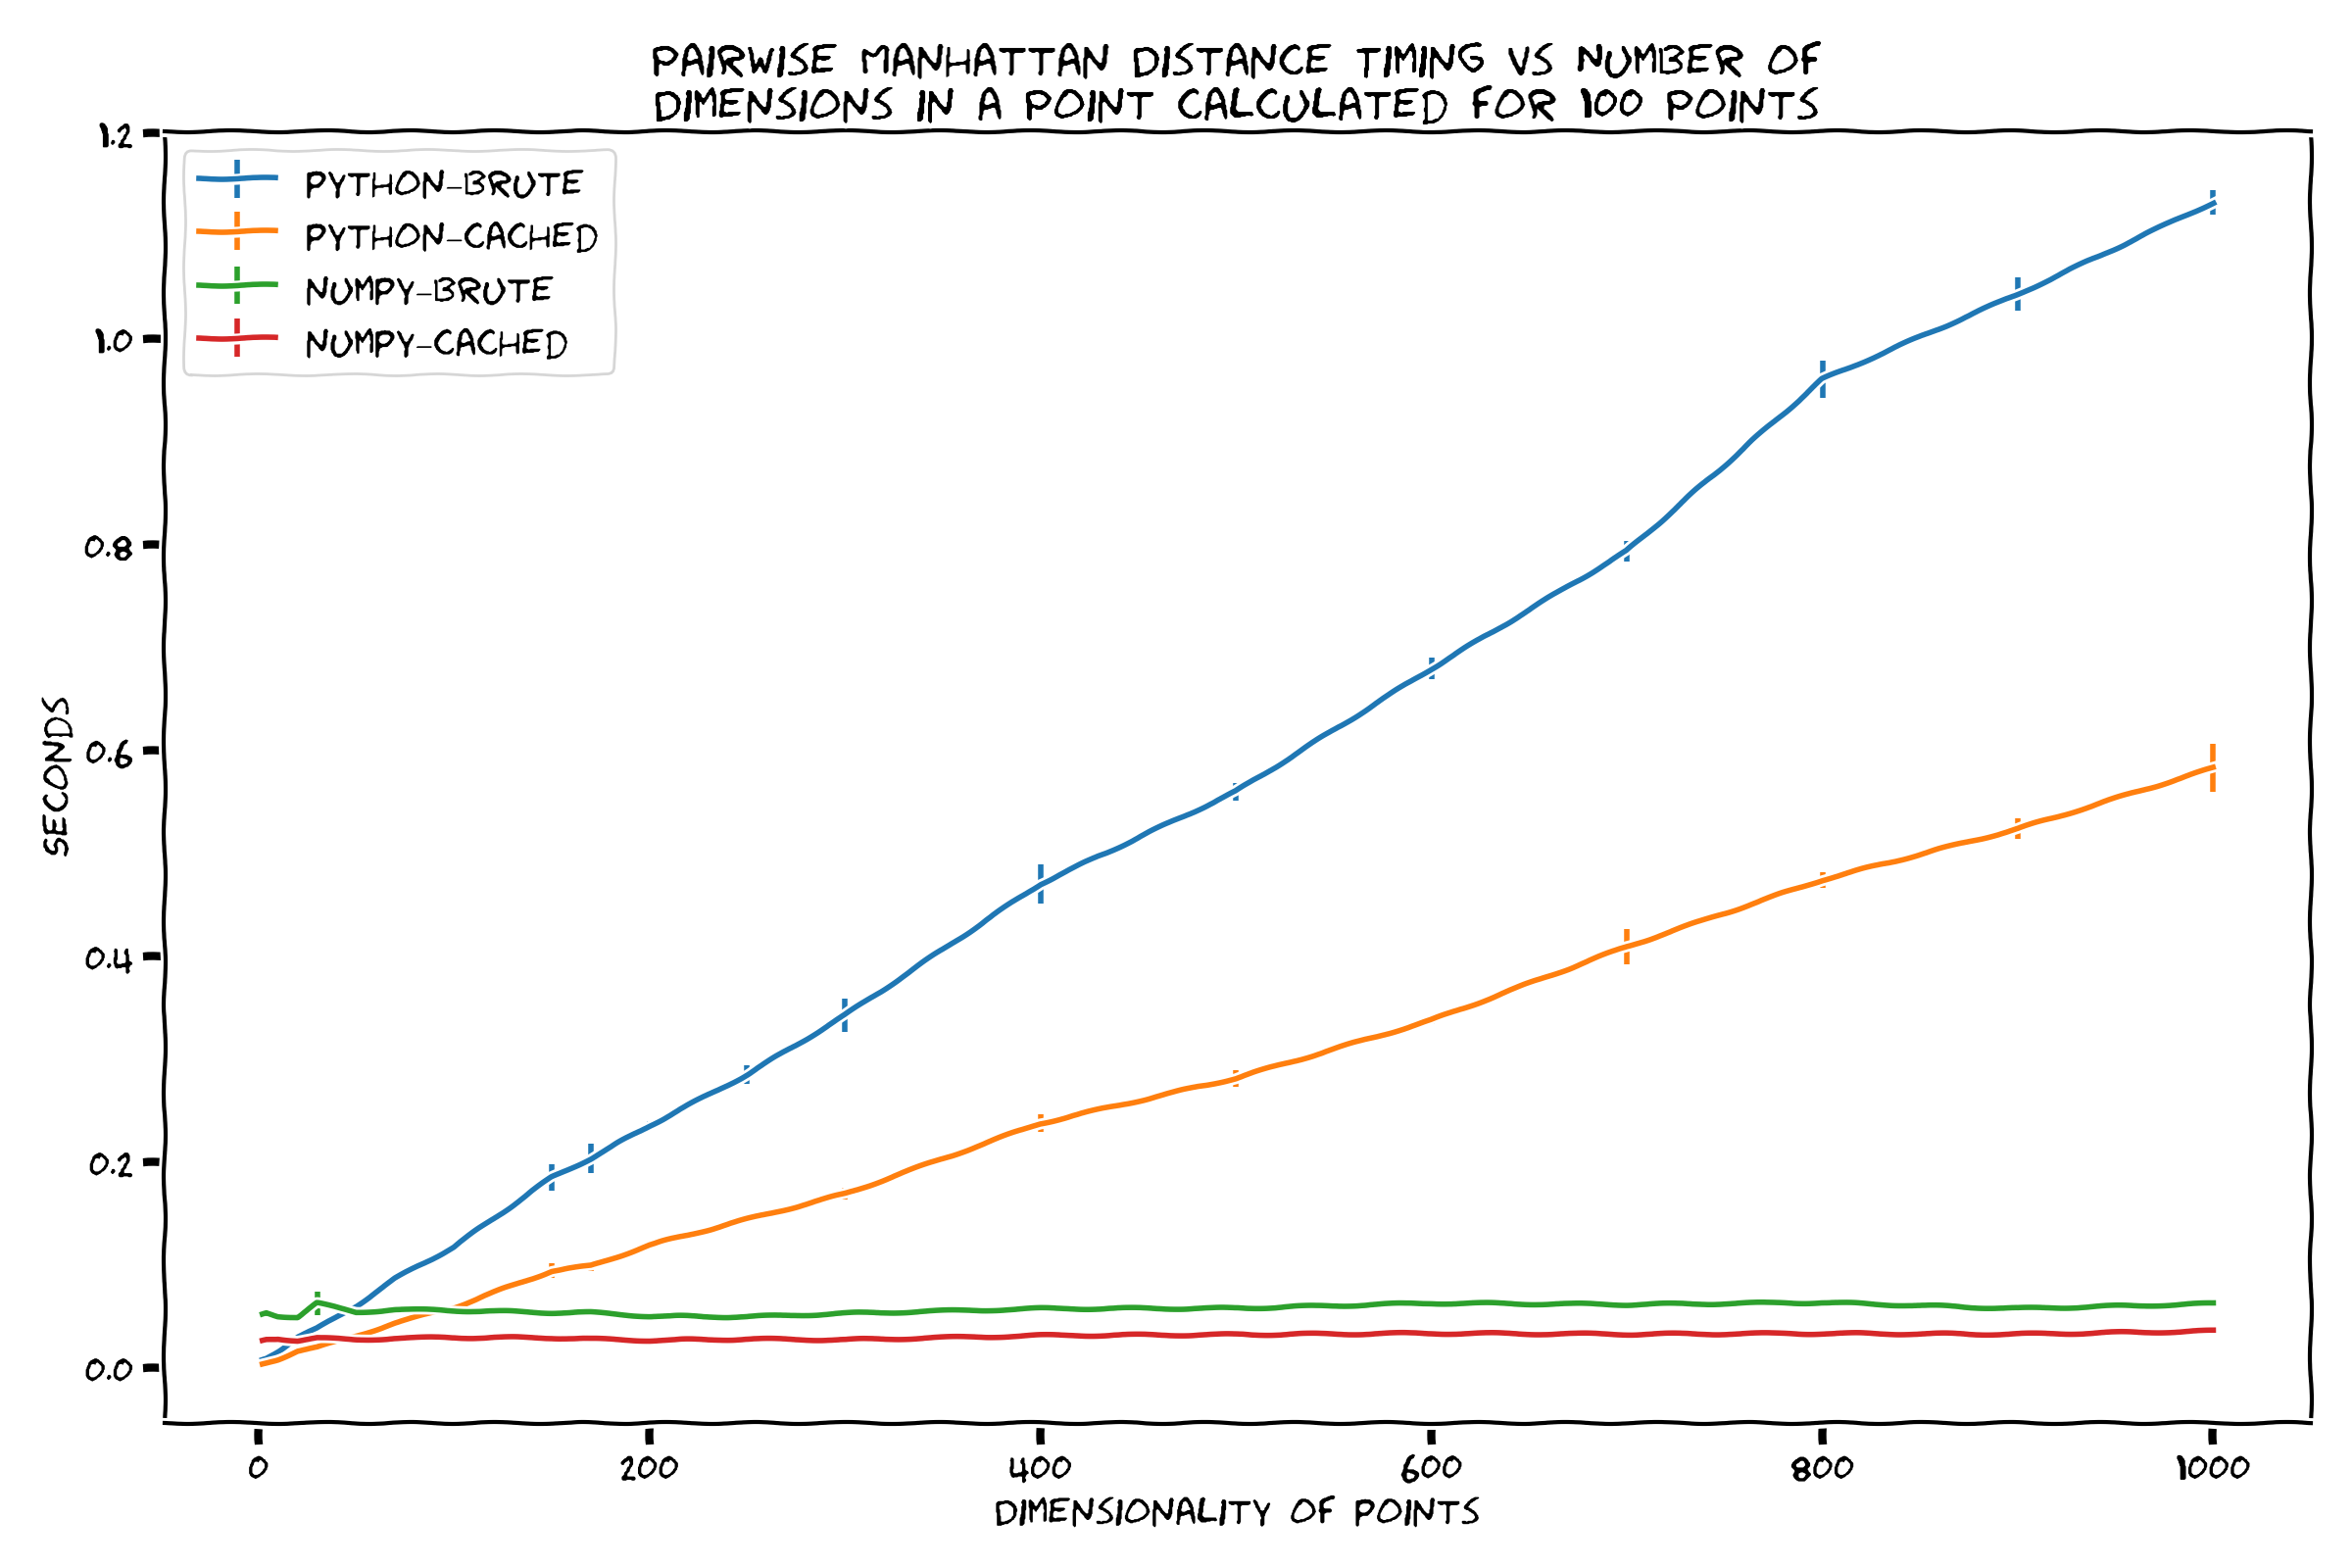
\includegraphics[width=0.98\paperwidth]{images/timing-vs-dims-at-100.png}
    }
    \note{
        \begin{itemize}
            \item This is a plot of the timing vs the number of dimentions in a point.
            \item Graphs created by running each implementation on randomly generated data (same data across implemetations) 5 times. The point it the mean of the times and the error bar is the standard dev of the times.
            \item For the \texttt{python\_brute} and \texttt{python\_cached} implementations we can see the predicted $\BigO(M)$ growth.
            \item At small input sizes we can see there is some overhead for converting lists into numpy that counteracts the
                advangate of vectorization
        \end{itemize}
    }
\end{frame}

\begin{frame}
    \makebox[\textwidth][c]{
        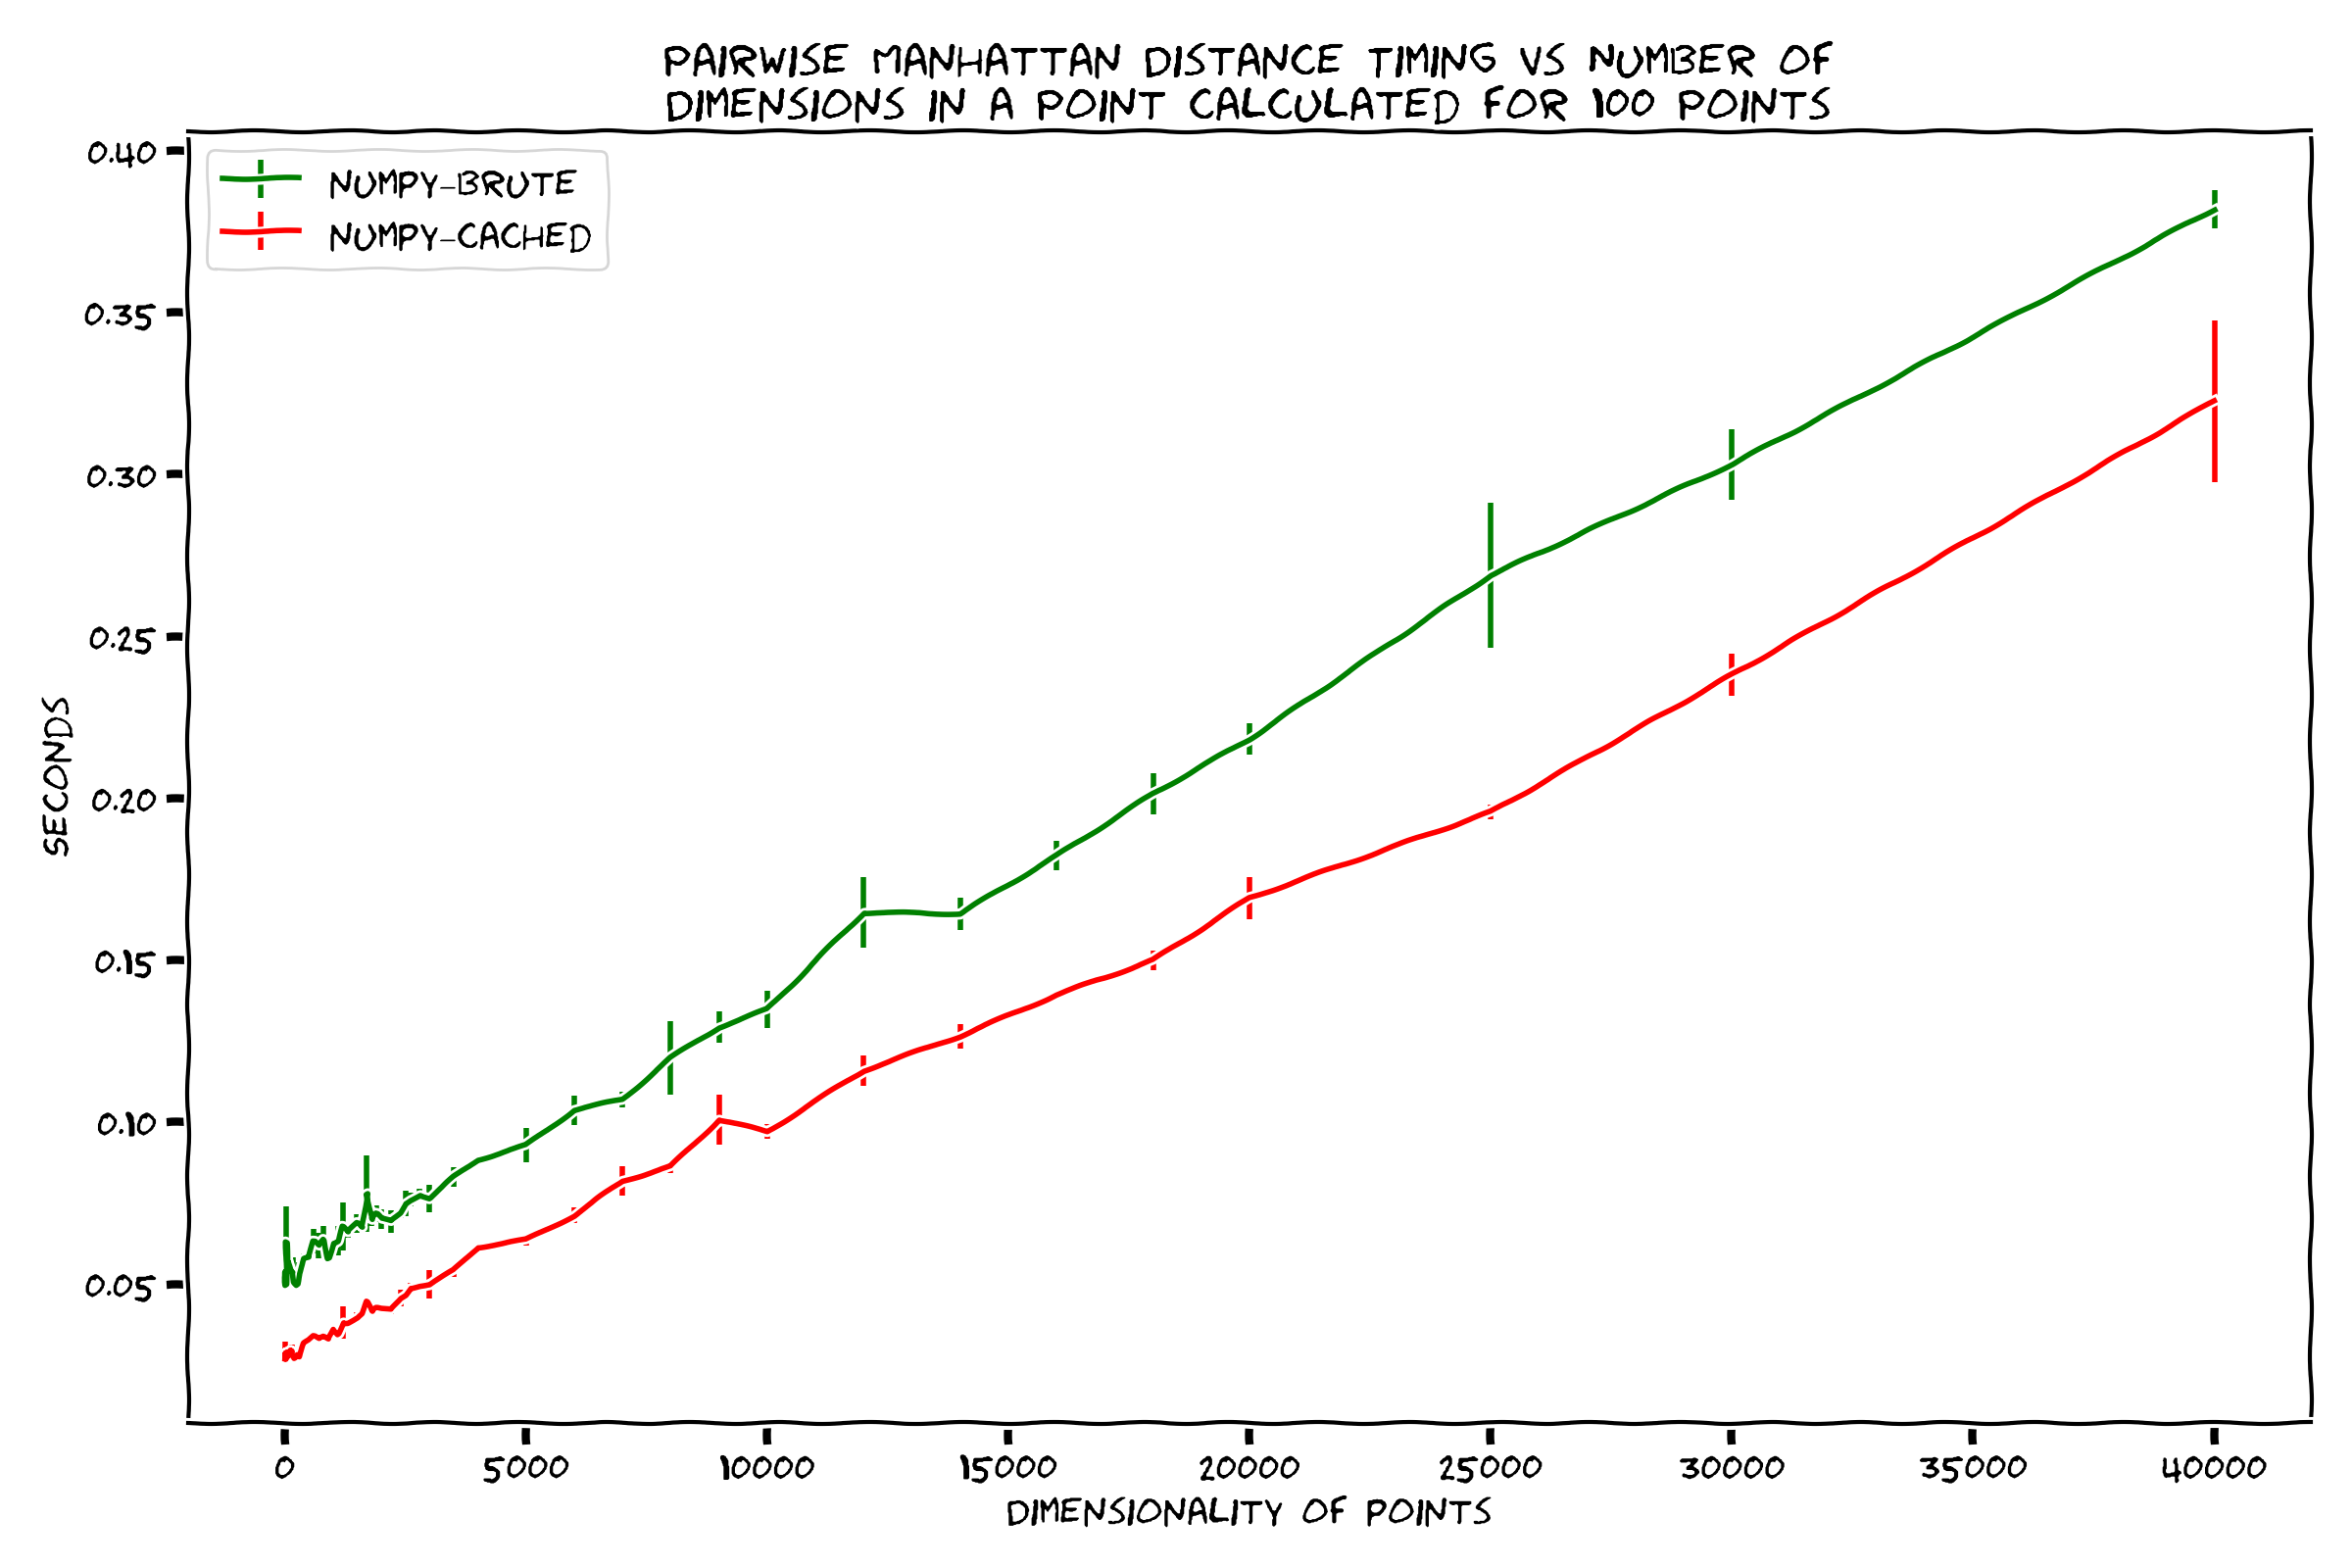
\includegraphics[width=0.98\paperwidth]{images/numpy-dims.png}
    }
    \note{
        \begin{itemize}
            \item Here we can see the same $\BigO(M)$ growth for numpy implemenetations where we have vectorized the manhattan distance
            \item This highlights how we are making computational improvments, not algorithmic ones
            \item I had to scale out to a lot more points to see this trend because when python code is in the graph it looks flat
            \item Note the very different scale on the y-axis
        \end{itemize}
    }
\end{frame}

\begin{frame}<1>[fragile,label=numpy_v3]
    \frametitle{Numpy Broadcast}

    \begin{pythoncode}
def pairwise_manhattan_numpy_v3(points: np.ndarray) -> np.ndarray:
    results = []
    for i in range(len(points)):
        results.append(np.sum(np.abs(points[i] - points), axis=1))
    return np.stack(results)
    \end{pythoncode}
    \note<1>{
        \begin{itemize}
            \item We can see that one of the loops is gone!
            \item If you guessed the answer is vectorization you are right
            \item This is specifically the idea of broadcasting which help you vectorize code
        \end{itemize}
    }
    \note<2>{
        \begin{itemize}
            \item points i is $\in \R^M$
            \item points is $\in \R^{N \text{ x } M}$
            \item The result of broadcasting vectorization for points is \texttt{[N, M]}
            \item There is this new kwarg for \texttt{np.sum}, \texttt{axis}
            \item This is a way to apply reductions to multi dimensional inputs
        \end{itemize}
    }
    \note<3>{
        \begin{itemize}
            \item Reducing \texttt{[N, M]} over axis 1 gives us \texttt{N}
            \item Results is a list of vectors of size $N$
            \item \texttt{np.stack} puts them on top of each other to form a single matrix
            \item Side Note: Type hints for array shapes has no support which sucks. To make broadcasting work you often need specific shapes but you can't communicate these constraints via type hints
        \end{itemize}
    }
    \note<4>{
        \begin{itemize}
            \item One thing to notice here is that we are back to doing redundant computation by calculating all pairs of points!
            \item It is possible to remove this redundency but it will get a little weird
        \end{itemize}
    }
\end{frame}

\begin{frame}
    \frametitle{Broadcasting}
    \begin{itemize}
        \item<1-> Vectorization can speed up code
        \item<2-> But what do I do when the shapes don't match?
        \item<3-> If i want to add a scalar to a vector do I have to copy the scalar into a vector to vectorize it?
        \item<4-> Broadcasting to the rescue!
    \end{itemize}
    \note<3->{
        \begin{itemize}
            \item Copying would be a waste of memory (need to have the scalar multiple times) and computation (time taken to make the copies of the scalar)
        \end{itemize}
    }
\end{frame}

\begin{frame}[fragile]
    \frametitle{Roll Your Own Broadcasting}
    \begin{pythoncode}
        def add_scalar_to_vector(scalar, vector):
            return [v + scalar for v in vector]
    \end{pythoncode}
    \note{
        \begin{itemize}
            \item The scalar is added to each element in the vector as if the scalar was expanded to a vector and a normal vectorized add was done.
        \end{itemize}
    }
\end{frame}

\begin{frame}
    \frametitle{Broadcasting Rules}
    \begin{enumerate}
        \item If there is a mismatch in the number of dimensions the shape with fewer is padded with $1$s on its leading side.
            \begin{itemize}
                \item $2 \text{ x } 3 + 3 \rightarrow 2 \text{ x } 3 + 1 \text{ x } 3$
            \end{itemize}
        \item If the size of some dimension doesn't match and one of the sizes is $1$ it is repeated to match the other size.
            \begin{itemize}
                \item $5 \text{ x } 4 + 5 \text{ x } 1 \rightarrow 5 \text{ x } 4 + 5 \text{ x } 4$
            \end{itemize}
        \item If there is a mismatch and neither size is $1$ an exception is thrown.
            \begin{itemize}
                \item $3 \text{ x } 4 + 4 \text{ x } 3 \rightarrow \text{ERROR}$
            \end{itemize}
    \end{enumerate}
\end{frame}

\begin{frame}
    \frametitle{Broadcasting Examples}
    \begin{center}
    \def\arraystretch{1.5}
    \begin{tabular}{ c c c c | c }
        $X \in \R^{2 \text{ x } 3}$ & $Y \in \R^{1 \text{ x } 3}$ & & $Y' \in \R^{2 \text{ x } 3}$ & $X + Y \in R^{2 \text{ x } 3}$ \\
        $
            \begin{bmatrix}
                1 & 2 & 3 \\
                4 & 5 & 6 \\
            \end{bmatrix}
        $
        &
        $
            \begin{bmatrix}
            1 & 2 & 1 \\
            \end{bmatrix}
        $
        &
        $\rightarrow$
        &
        $
            \begin{bmatrix}
            1 & 2 & 1 \\
            1 & 2 & 1 \\
            \end{bmatrix}
        $
        &
        $
            \begin{bmatrix}
                2 & 4 & 4 \\
                5 & 7 & 7 \\
            \end{bmatrix}
        $ \\
        & & & & \\
        $X \in \R^{2 \text{ x } 3}$ & $Z \in \R^{2 \text{ x } 1}$ & & $Z' \in \R^{2 \text{ x } 3}$ & $ X + Z \in R^{2 \text{ x } 3} $ \\
        $
            \begin{bmatrix}
                1 & 2 & 3 \\
                4 & 5 & 6 \\
            \end{bmatrix}
        $
        &
        $
            \begin{bmatrix}
            2 \\
            3 \\
            \end{bmatrix}
        $
        &
        $\rightarrow$
        &
        $
            \begin{bmatrix}
                2 & 2 & 2\\
                3 & 3 & 3\\
            \end{bmatrix}
        $
        &
        $
            \begin{bmatrix}
                3 & 4 & 5 \\
                7 & 8 & 9 \\
            \end{bmatrix}
        $ \\
    \end{tabular}
    \end{center}
    \note{
        \begin{itemize}
            \item Here we see examples of broadcasting
            \item The first one is broadcasting over the rows
            \item The second one is broadcasting over the columns
            \item Stress that these copies don't actually happen but computation acts like it did
        \end{itemize}
    }

\end{frame}

\againframe<2>{numpy_v3}

\begin{frame}
    \frametitle{Multidimensional Reduction}
    \begin{center}
        \texttt{y = np.sum(x)}
    \end{center}
    \begin{columns}
        \column{0.5\textwidth}
            $$ x \in \R^{4 \text{ x } 3} $$
            \[
            \begin{bmatrix}
            1 & 2 & 3 \\
            4 & 5 & 6 \\
            7 & 8 & 9 \\
            10 & 11 & 12 \\
            \end{bmatrix}
            \]
        \column{0.5\textwidth}
            $$ y \in \R $$
            \[
                78
            \]
    \end{columns}
    \note{
        \begin{itemize}
            \item We said before that a reduction turned a vector into a scalar, but what about a high dim?
            \item Without an axis to reduces the whole things, results in $78$
        \end{itemize}
    }
\end{frame}

\begin{frame}
    \frametitle{Reduction Along an Axis}
    \begin{center}
        \texttt{y = np.sum(x, axis=1)}
    \end{center}
    \begin{columns}
        \column{0.5\textwidth}
            $$ x \in \R^{4 \text{ x } 3} $$
            \[
            \overrightarrow{
            \begin{bmatrix}
            1 & 2 & 3 \\
            4 & 5 & 6 \\
            7 & 8 & 9 \\
            10 & 11 & 12 \\
            \end{bmatrix}
            }\]
        \column{0.5\textwidth}
            $$ y \in \R^4 $$
            \[
            \begin{bmatrix}
            6 \\
            15 \\
            24 \\
            33 \\
            \end{bmatrix}
            \]
    \end{columns}
    \note{
        \begin{itemize}
            \item The axis argument allows for a reduction that only reduces the number of dims by one
            \item Reduction over the axis 1 is applied across the columns for matrices resulting in a vector
        \end{itemize}
    }
\end{frame}

\begin{frame}
    \frametitle{Reduction Along an Axis}
    \begin{center}
        \texttt{y = np.sum(x, axis=0)}
    \end{center}
    \begin{columns}
        \column{0.5\textwidth}
            $$ x \in \R^{4 \text{ x } 3} $$
            \[
            \tikz[remember picture, baseline=(mat.center)]{\node[inner sep=0](mat){$\begin{bmatrix} 
            1 & 2 & 3 \\
            4 & 5 & 6 \\
            7 & 8 & 9 \\
            10 & 11 & 12 \\
            \end{bmatrix}$};}
            \begin{tikzpicture}[overlay,remember picture,>=Triangle]
            \draw[black,thick,->] node[anchor=north east,align=left, inner xsep=0pt] (nn2) at (mat.north west) {} (nn2.south) -- (nn2.south|-mat.south);
            \end{tikzpicture}
        \]
        \column{0.5\textwidth}
            $$ y \in \R^3 $$
            \[
            \begin{bmatrix}
            22 & 26 & 30 \\
            \end{bmatrix}
            \]
    \end{columns}
    \note{
        \begin{itemize}
            \item Reduction over axis 0 is applied across the rows for matrices
            \item There is also a \texttt{keepdims} argument to keep the sinlge dimension of size 1 so instead of getting a vector of size $3$ you get one of size \texttt{[1, 3]}
        \end{itemize}
    }
\end{frame}

\againframe<3->{numpy_v3}

\begin{frame}[fragile]
    \frametitle{Numpy Broadcast Cached}

    \begin{pythoncode}
def pairwise_manhattan_numpy_broadcast_cached(
    points: np.ndarray
) -> np.ndarray:
    results = np.zeros((len(points), len(points)), dtype=np.int32)
    dists = []
    for i in range(len(points)):
        dists.append(np.sum(np.abs(points[i] - points[i:]), axis=1))
    for i, dist in enumerate(dists):
        results[i, i:] = dist
    return results + results.T
    \end{pythoncode}
    \begin{itemize}
        \item<2-> Still $\BigO(N^2M)$ runtime.
        \item<2-> Still $\BigO(N^2)$ memory.
    \end{itemize}
    \note<1>{
        \begin{itemize}
            \item Here we are back to preallocating our results
            \item When we compute the distances we only compute before by slicing the points matrix
            \item We get back a list of tensors that are not the same shape (each one is on smaller than the previous)
            \item In python we copy these into the regular matrix so that it is a upper triangular matrix
            \begin{itemize}
                \item Upper triangular matrix means it only has values above the diagonal
                \item Only value when the column index $j$ is $\ge$ the row index $i$
            \end{itemize}
        \item We transpose (the rows become columns and columns rows) and add. Because we are upper triangle (lower values are all zero) the add just copies upper values in
            \item This would double the diag values but because we know Manhattan distance is $0$ with ourselves the diag will stay $0$
        \end{itemize}
    }
    \note<2>{
        \begin{itemize}
            \item We are adding a loop over the N points (copying the values into the results) $\BigO(N)$
            \item The addition is $\BigO(N^2)$
            \item Whole thing is $\BigO(N^2M + N^2 + N)$ but we can throw away extra for Big-O
            \item Even though we have slow python loops at large values we are saving so much computation it is worth it
            \item Sometimes a strange mix of vectorized and python is the best way.
        \end{itemize}
    }
\end{frame}

\begin{frame}<-2>[fragile,label=double]
    \frametitle{Numpy Double Broadcast}

    \begin{pythoncode}
def pairwise_manhattan_numpy_v4(points: np.ndarray) -> np.ndarray:
    exp_points = np.expand_dims(points, 1)  # [N, 1, M]
    return np.sum(np.abs(exp_points - points), axis=-1)
    \end{pythoncode}
    \begin{itemize}
        \item<3->Still $\BigO(N^2M)$ in runtime
        \item<3->Now $\BigO(N^2M)$ in memory
    \end{itemize}
    \note<1>{
        \begin{itemize}
            \item All the loops are gone!
            \item We add a dimension of size $1$ into the points
            \item When we do the subtraction the points \texttt{[N, M]} is expanded to \texttt{[1, N, M]}
            \item \texttt{[N, 1, M]} + \texttt{[1, N, M]} $\rightarrow$ \texttt{[N, N, M]}
            \item Reduction over axis $-1$ (same as negative indexing in python, sum over the last dim)
            \item Reduction gives us \texttt{[N, N]} aka our answer
        \end{itemize}
    }
    \note<2>{
        \begin{itemize}
            \item Now that we are double broadcasting there is no way to express the fact that we can skip the repeated work of calculating the distance between symmetric pairs of points.
        \end{itemize}
    }
    \note<3->{
        \begin{itemize}
            \item We are going to revisit Big-O for this implementation
            \item The runtime is still the same, remember the loops are still there, they are just in C not python
            \item We have this itermediate result of size \texttt{[N, N, M]} so our memory usage is higher. $\BigO(N^2M)$
        \end{itemize}
    }
\end{frame}

\begin{frame}<1>[label=micro]
    \frametitle{Broadcasting Micro Benchmark}
    \makebox[\textwidth][c]{
        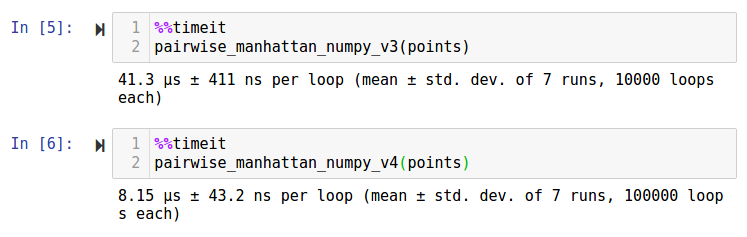
\includegraphics[width=0.9\paperwidth]{images/microbenchmark-broadcast.png}
    }
    \note<1>{
        \begin{itemize}
            \item This was a promising implementation in the thread
            \item Here we can see on a small micro bench mark (4 points of dim 2) that shows a lot of promise
            \item As I scaled it out speeds weren't meaningfully different/were worse from the single broadcast
            \item Lets look at why it was worse
        \end{itemize}
    }
    \note<2>{
        \begin{itemize}
            \item Due to memory usage this is actually slower than the previous solutions
            \item When you run out of memory you start swapping which involves disk and is therefore super slow
            \item Due to memory usage I could only get this version to work for limited points and only a few dimensions.
            \begin{center}
            \begin{tabular}{| r | r || r | r |}
                \hline
                points & dims & Single Memory & Double Memory \\
                \hline
                10000 & 2 & 381.47MiB & 762.94MiB \\
                \hline
                10000 & 10 & & 3.73GiB \\
                \hline
                10000 & 150 & & 55.88GiB \\
                \hline
                80000 & 2 & 23.84GiB & 47.68GiB \\
                \hline
                80000 & 150 & & 3.49PiB\\
                \hline
            \end{tabular}
            \end{center}
            \item This is an exmaple of why it is important to benchmark in a realistic scenario.
        \end{itemize}
    }
\end{frame}

\againframe<3>{double}

\againframe<2>{micro}

\end{subsection} %NumPy

\begin{subsection}{Cython}

\begin{frame}<1>[fragile,label=cython]
    \frametitle{Cython Implementation}
    \begin{cythoncode}
@cython.wraparound(False)
@cython.boundscheck(False)
cpdef int[:, :] pairwise_manhattan(int[:, :] points):
    cdef int n = points.shape[0]
    cdef int m = points.shape[1]
    results = np.zeros((n, n), dtype=np.int32)
    cdef int[:, :] results_view = results
    cdef int i, j, k, dist
    for i in range(n):
        for j in range(i, n):
            dist = 0
            for k in range(m):
                dist += abs(points[i, k] - points[j, k])
            results_view[i, j] = dist
            results_view[j, i] = dist
    return results
    \end{cythoncode}
    \note<1>{
        \begin{itemize}
            \item The cython code looks complex but if we zoom in we can see it looks a lot like our original python code
            \item There are a lot of annotations that help speed things up.
            \item we can just write loops, we don't have to think about vectorization
        \end{itemize}
    }
    \note<2->{
        \begin{itemize}
            \item There are a lot of optimizations left of the table, for example operating on batch points at a time in the inner loops for better cache coherence
            \item we could skip computing the distance to ourselves because we know it is zero
            \item These kind of optimizations are very hard (impossible) to express with NumPy
            \item We didn't use it but Cython also supports defining objects and structs which makes it amenable to speeding up code that isn't all numeric arrays
            \item NumPy is basically array only if you want speed.
    \end{itemize}
    }
\end{frame}

\begin{frame}[fragile]
    \frametitle{Cython Decorators}
    \begin{cythoncode}
    @cython.wraparound(False)
    @cython.boundscheck(False)
    \end{cythoncode}
    \note{
        \begin{itemize}
            \item These are directives that tell cython how to compile code
            \item \texttt{wrapsround} turns off the ability to do negative indexing
            \item \texttt{boundscheck} turns off rasing an error when you access past the end of an array
            \item Both of these ease of use thing require the length of the array. C arrays don't carry their lengths so we need to ask the python object for the length. Accessing python objects are slow and require the GIL
        \end{itemize}
    }
\end{frame}

\begin{frame}[fragile]
    \frametitle{Cython Function Definition}
    \begin{cythoncode}
    cpdef int[:, :] pairwise_manhattan(int[:, :] points):
    \end{cythoncode}
    \note{
        \begin{itemize}
            \item \texttt{cpdef} is a utility to make this function callable by python code and other cython code. C function calls are faster and there is slight overhead from the \texttt{cpdef}. Cython in a tight inner loop (like a function of manhattan distance) should use \texttt{cdef}
            \item \texttt{int[:, :]} before the function name is the return type
            \item It is also a type of the input (points)
            \item We will get to what the types are in a second
        \end{itemize}
    }
\end{frame}

\begin{frame}<-2>[fragile,label=declare]
    \frametitle{Cython Variable Declaration}
    \begin{cythoncode}
        cdef int n = points.shape[0]
        cdef int m = points.shape[1]
        results = np.zeros((n, n), dtype=np.int32)
        cdef int[:, :] results_view = results
        cdef int i, j, k, dist
    \end{cythoncode}
    \note<1>{
        \begin{itemize}
            \item \texttt{cdef} is used to statically declare variables. This tells the compiler what the type is so it can compile it to C.
        \end{itemize}
    }
    \note<2>{
        \begin{itemize}
            \item \texttt{results} is a dynamically created numpy array, it it known to the python interpreter, the gil is needed to make it, the ref counter is incremented by one when we make it, and it is a python object that will be safe to use in python after we return it. Making dynamic python objects so easily is a strength of cython.
        \end{itemize}
    }
    \note<3>{
        \begin{itemize}
            \item \texttt{int[:, :]} is a typed memoryview
            \item a type memoryview is a view of the memory that backs an object that supports the buffer interface
            \item the buffer interface specific way that an object lays out its data in memory so other things can access the content. Things like NumPy arrays and the stdlib array class support this interface
            \item \texttt{results\_view} is a typed memory view of the memory that holds the underlying data of results. This view lets us access the object from C, without gil
        \end{itemize}
    }
\end{frame}

\begin{frame}
    \makebox[\textwidth][c]{
        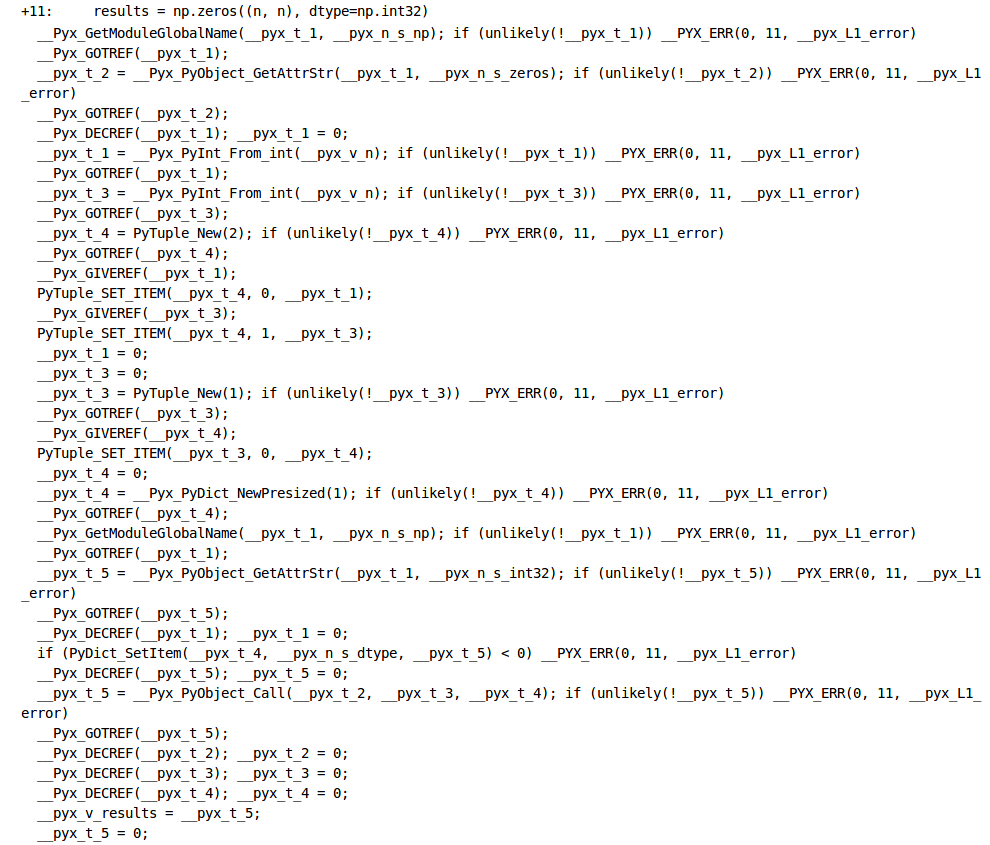
\includegraphics[width=0.98\paperwidth]{images/create-python-object.png}
    }
    \note{
        \begin{itemize}
            \item Here we can see some of the code that is generated when creating the results python object. Having to interface with the CPython API like this would be difficult without cython
        \end{itemize}
    }
\end{frame}

\againframe<3>{declare}

\begin{frame}[fragile]
    \frametitle{Cython Manhattan Distance}
    \begin{cythoncode}
    from libc.stdlib cimport abs
    cimport cython

    @cython.wraparound(False)
    @cython.boundscheck(False)
    cdef inline int manhattan_distance(int[:] x, int[:] y):
        cdef int i
        cdef int m = x.shape[0]
        cdef int dist = 0
        for i in range(m):
            dist += abs(x[i] - y[i])
        return dist
    \end{cythoncode}
    \note{
        \begin{itemize}
            \item I didn't do this in the code so it looks like the others but I would if this was real production code.
            \item cdef means this is only callable from cython but it has fast C function calls instead of slow python calls
            \item the inline keyword means when this is complied this code is directly insearted, not called as a function
            \item This gives us the speed of having code inline but the reusablilty/nice SWE practice of having a seperate function for it.
            \item We import \texttt{abs} from the C standard library so we always use the C version, if not cython will swap the version (C vs python) based on the datatypes and we wouldn't be able to release the GIL
        \end{itemize}
    }
\end{frame}

\againframe<2>{cython}

\end{subsection} %Cython
\end{section} %Implementation

\begin{section}{Results}

\begin{frame}
    \makebox[\textwidth][c]{
        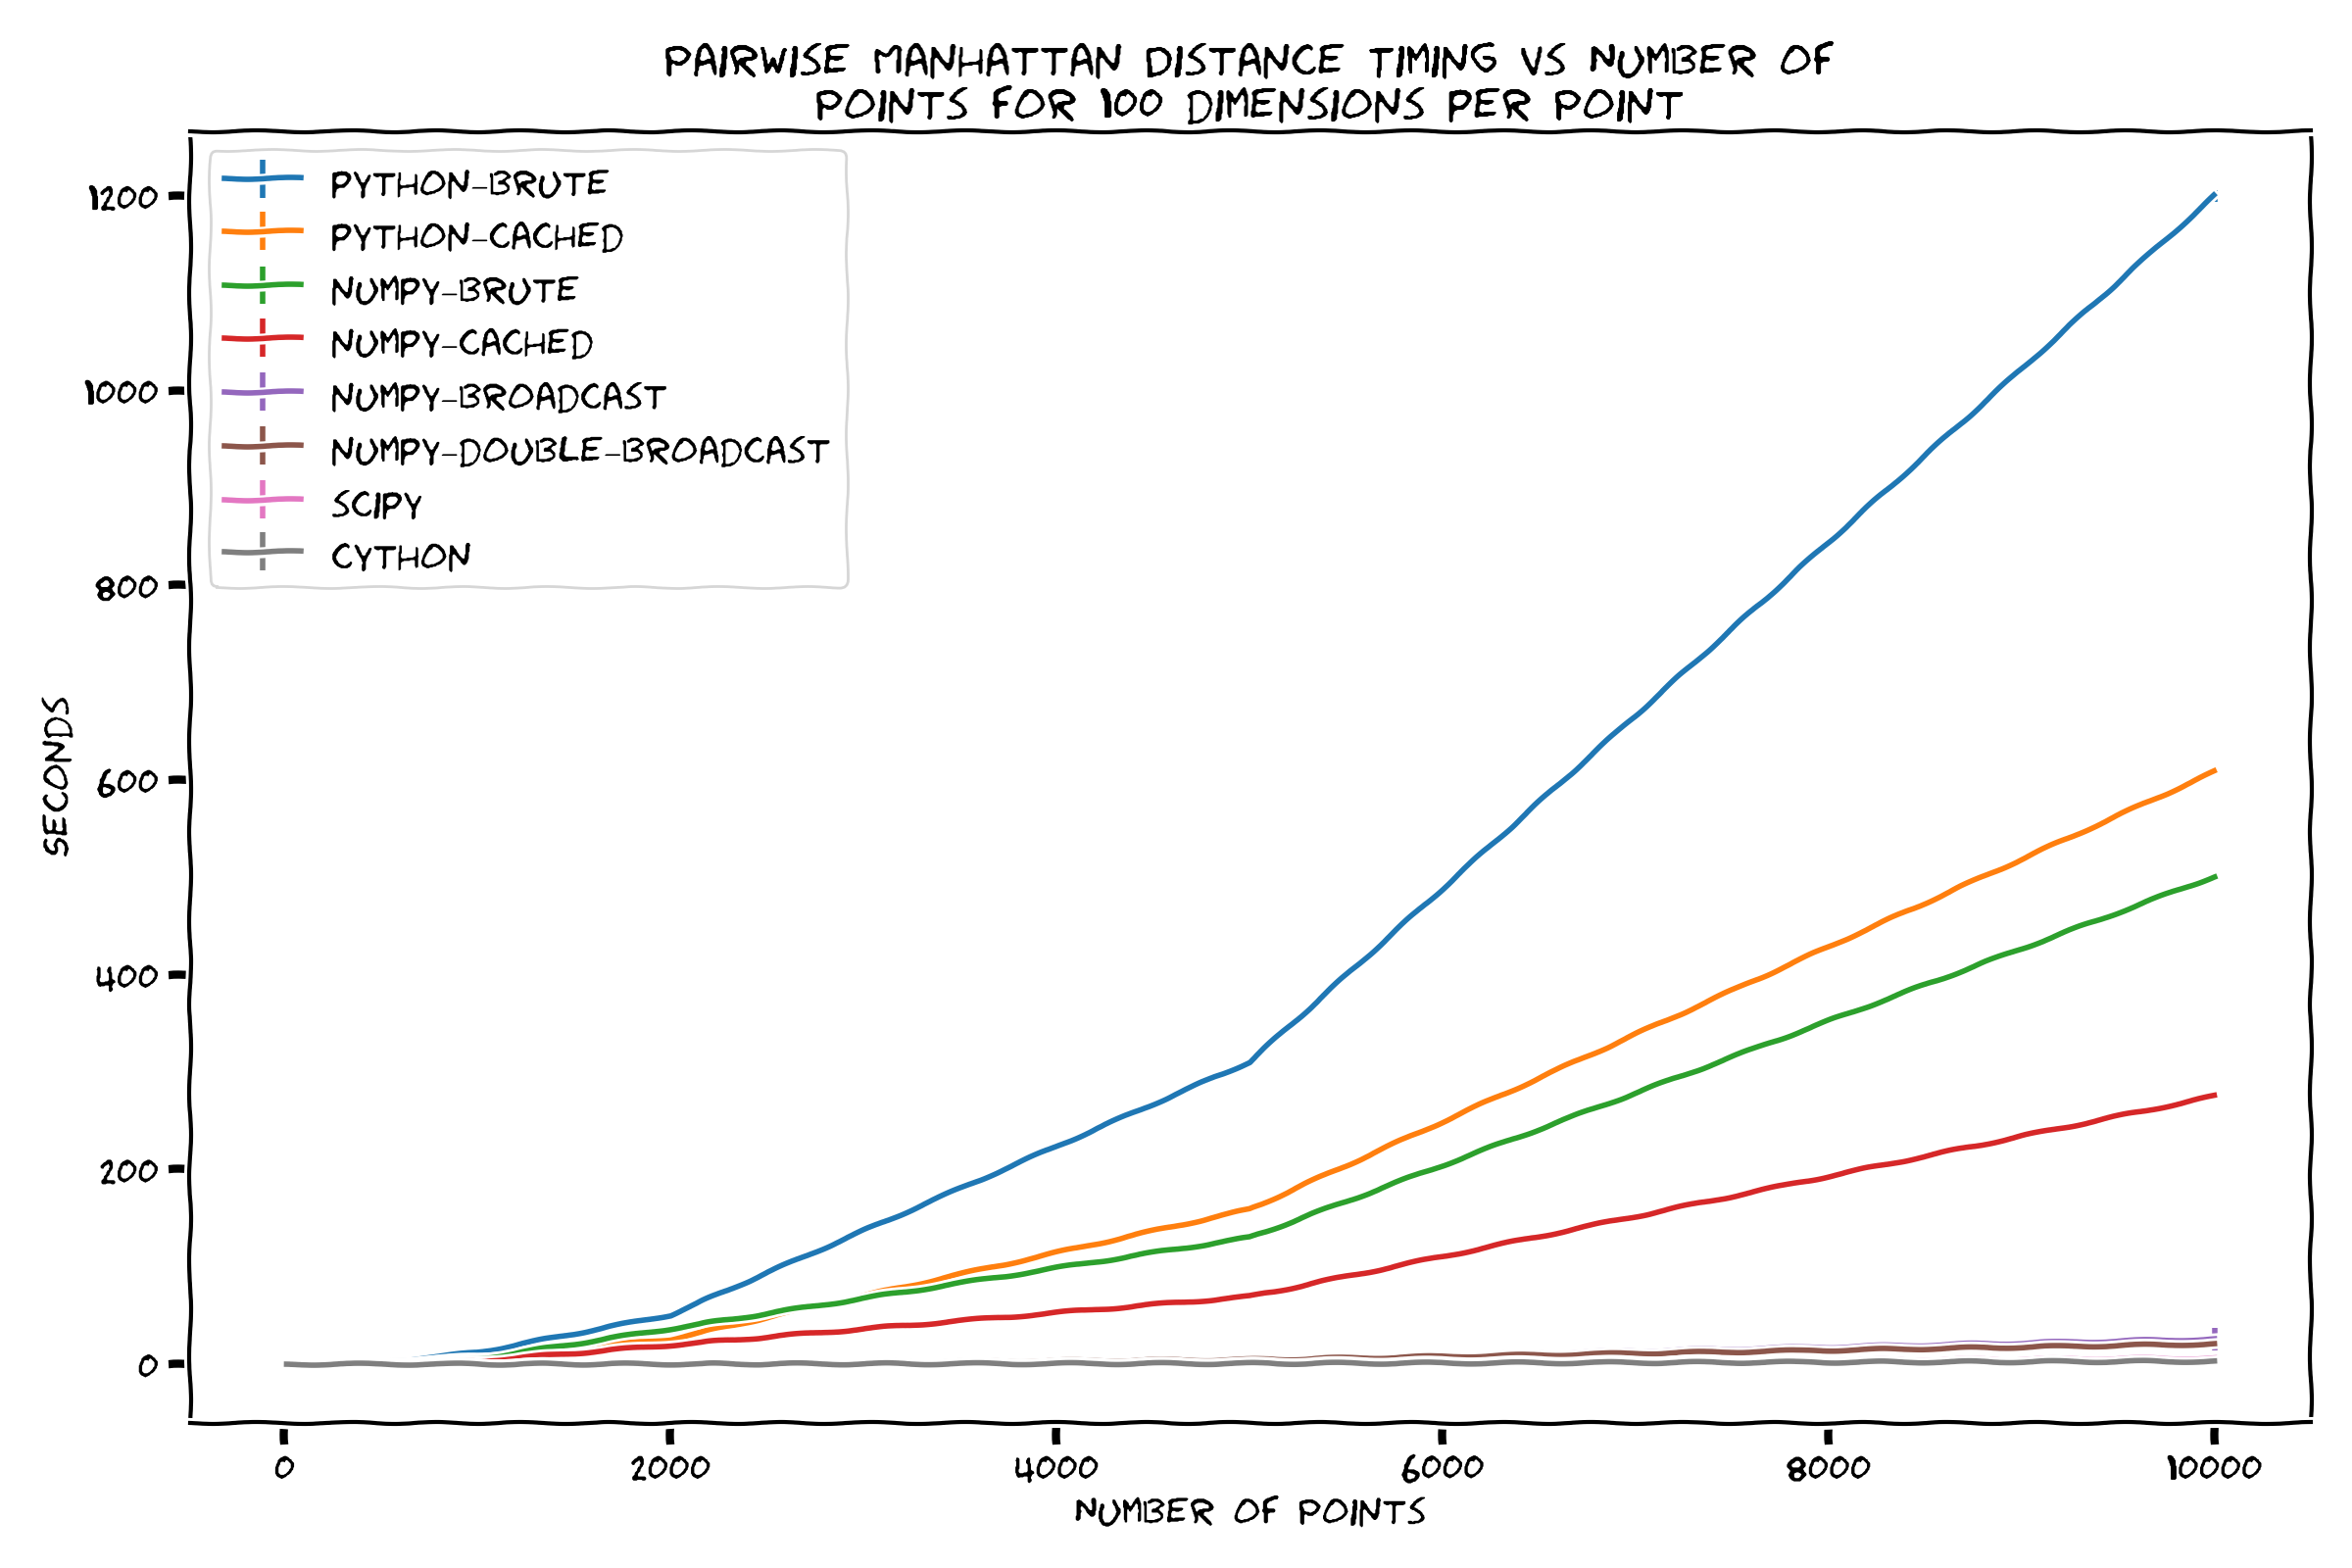
\includegraphics[width=0.98\paperwidth]{images/timing-vs-points-10000-all-impls.png}
    }
    \note{
        \begin{itemize}
            \item Here we can see the timing curves of various implemetations as we scale up the number of points.
            \item We can see the $\BigO(N^2M)$ growth for our algos
            \item The numpy broadcasting, scipy, and cython solutions are hard to see, we'll zoom in
            \item SciPy is a set of more specific/advanced scientific functions that includes a manhattan distance function
        \end{itemize}
    }
\end{frame}

\begin{frame}
    \makebox[\textwidth][c]{
        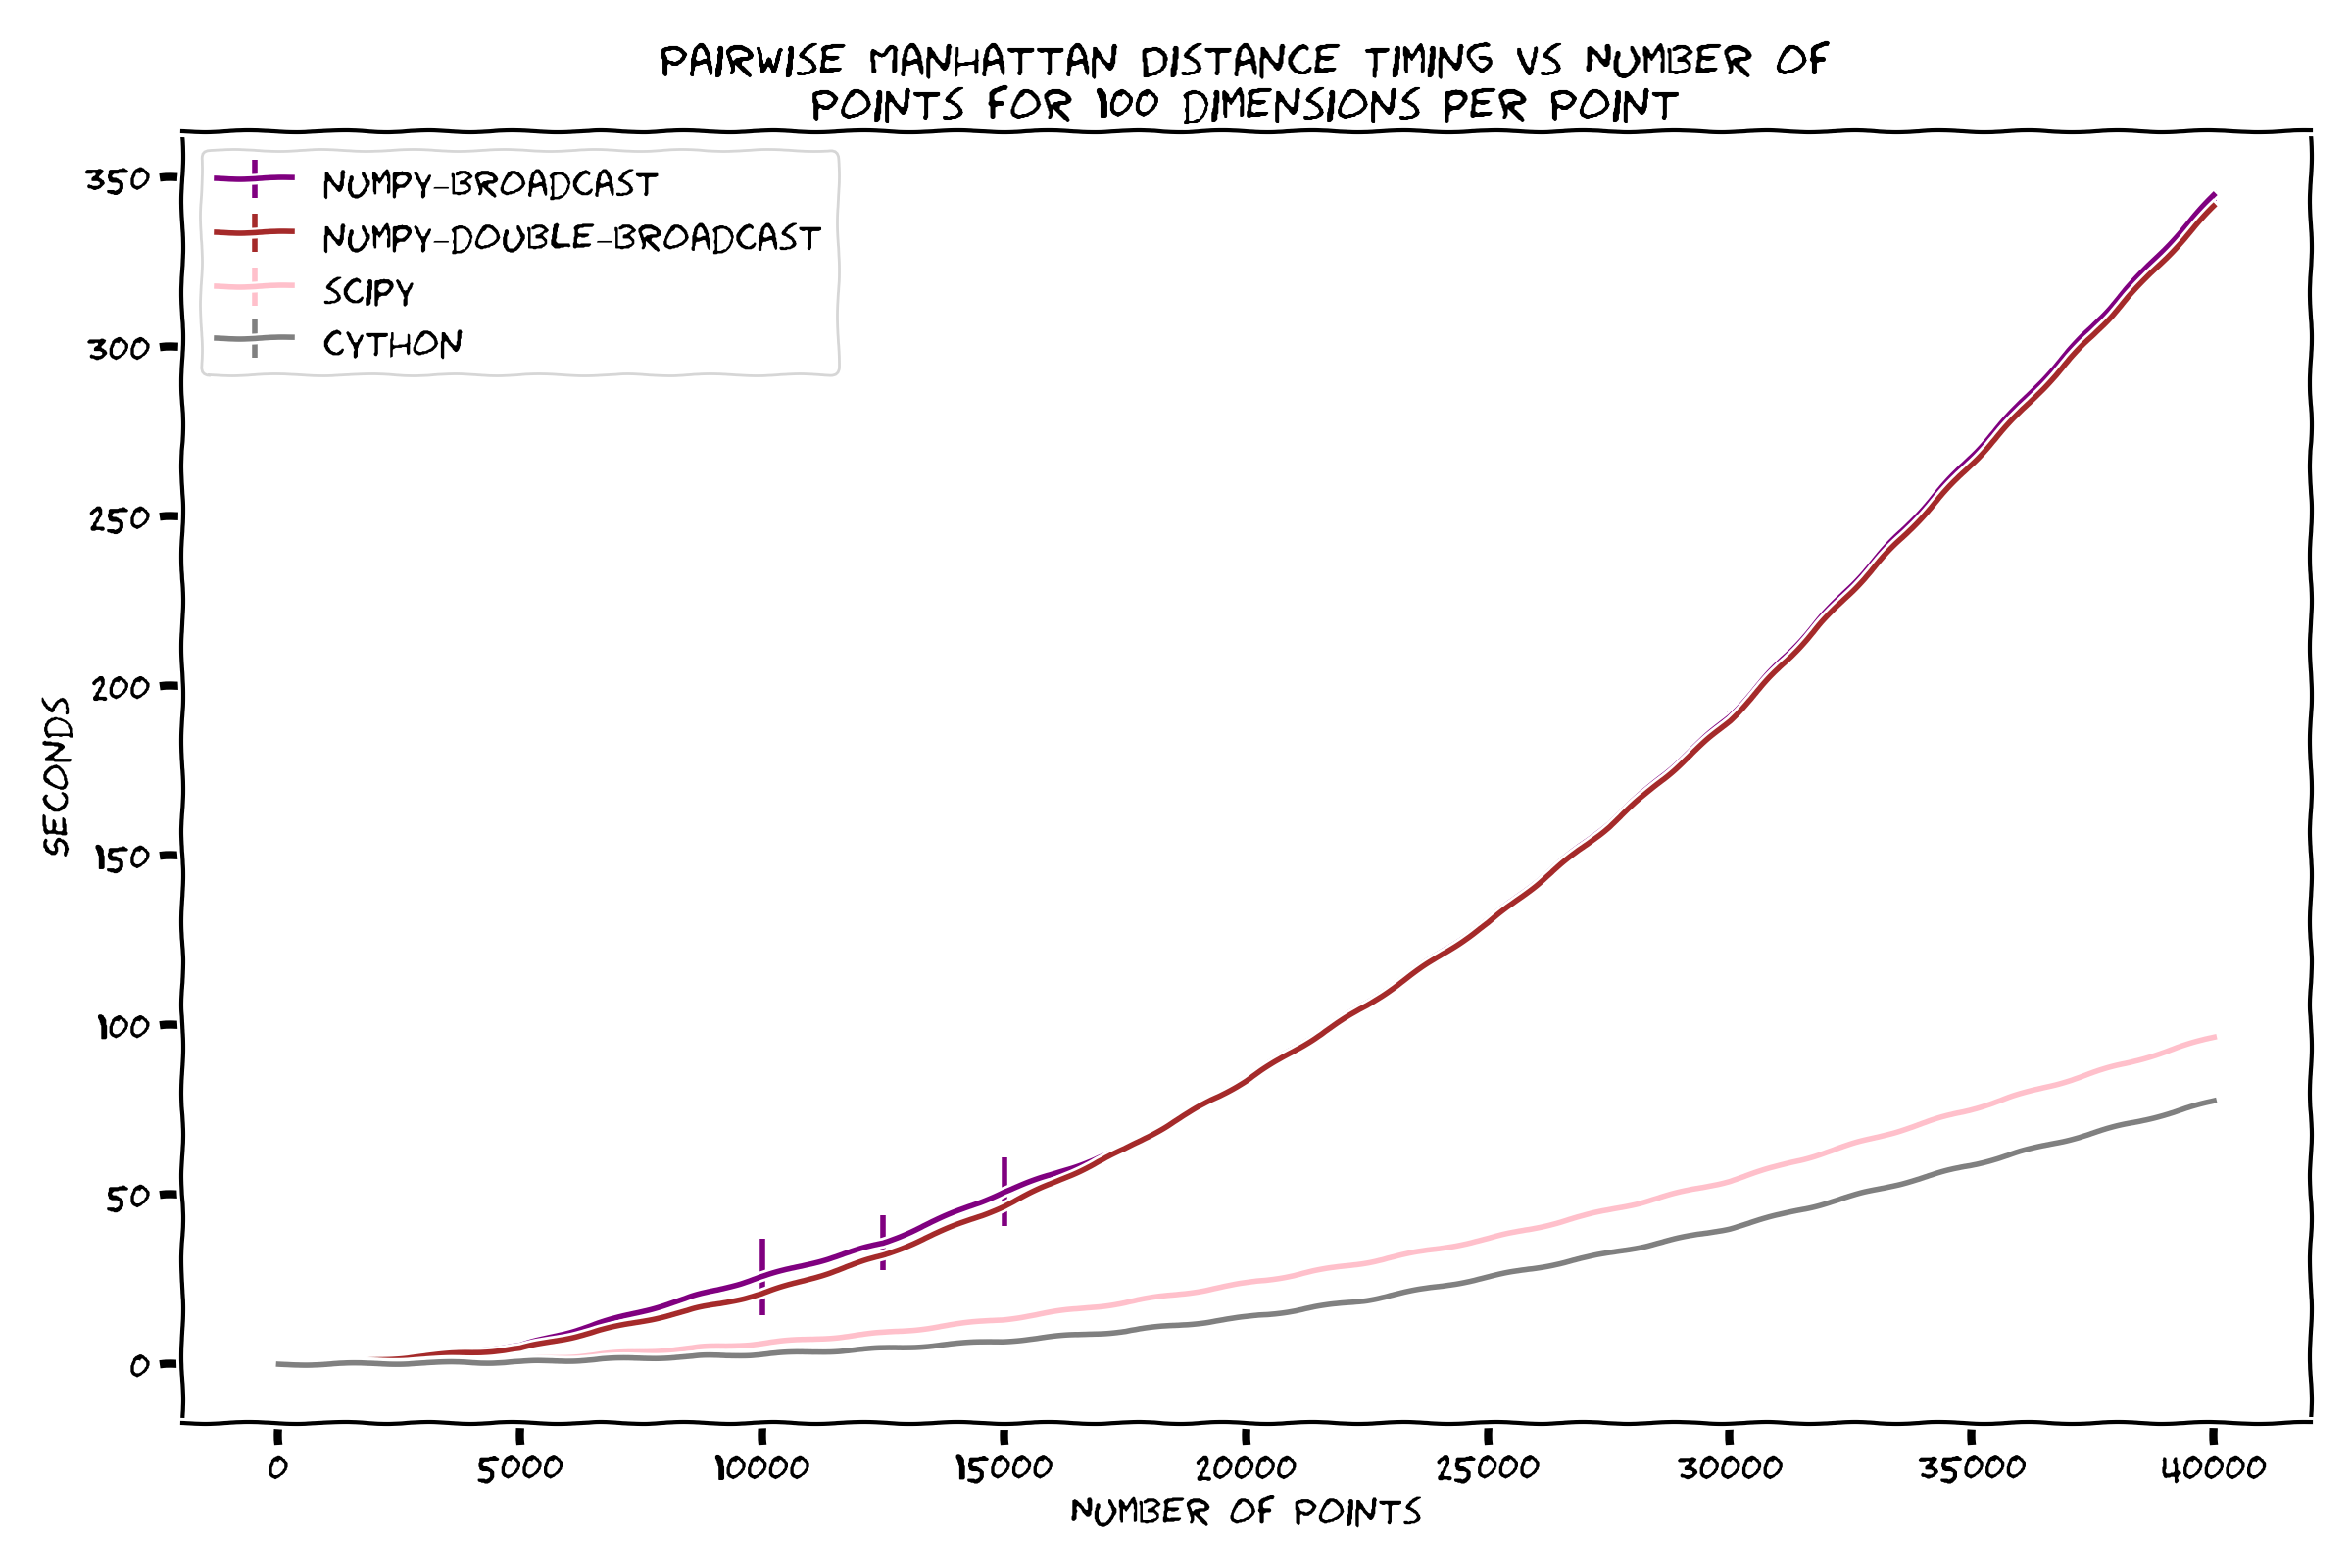
\includegraphics[width=0.98\paperwidth]{images/timing-vs-points-40000-some-impls.png}
    }
    \note{
        \begin{itemize}
            \item Here we are looking at only some implementations
            \begin{itemize}
                \item \texttt{numpy\_broadcast}
                \item \texttt{numpy\_broadcast\_cached}
                \item \texttt{scipy}
                \item \texttt{cython}
            \end{itemize}
            \item As mentioned earlier the double broadcasting solution didn't show meaningful gains over the broadcasting and I actually couldn't get it to run with 100 dimensional points.
            \item We can start to see the $\BigO(N^2M)$ growth
        \end{itemize}
    }
\end{frame}

\begin{frame}
    \makebox[\textwidth][c]{
        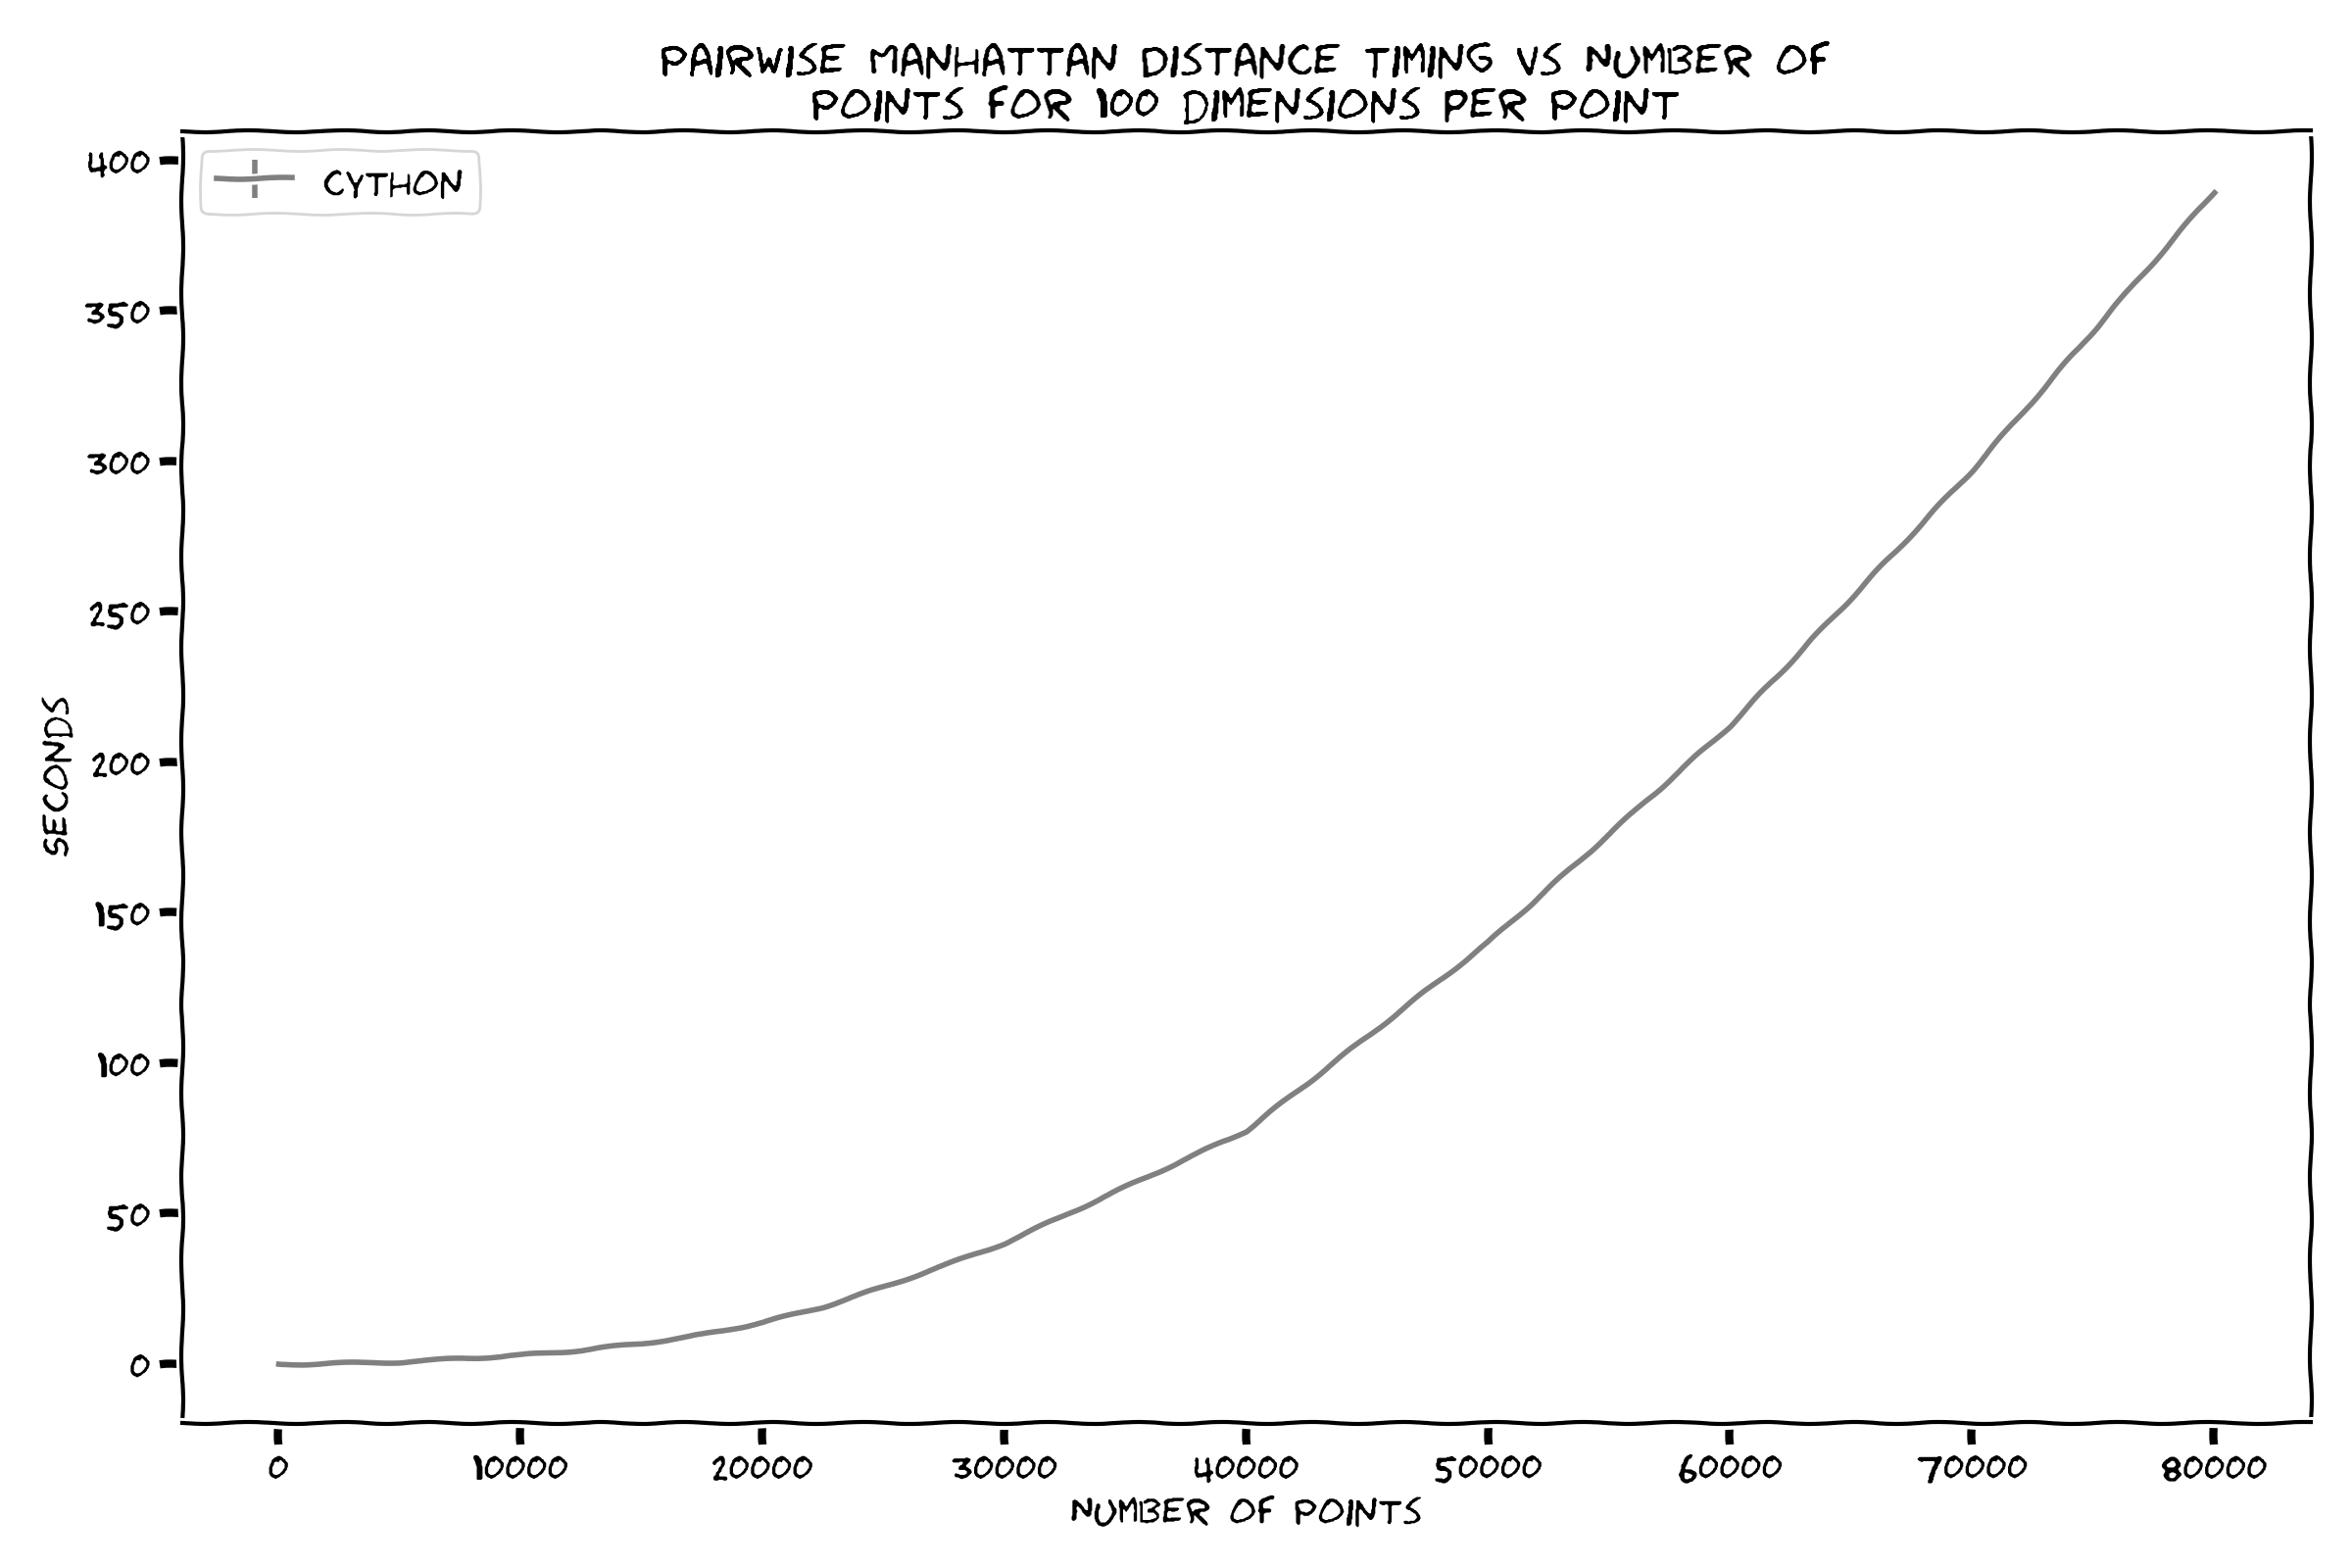
\includegraphics[width=0.98\paperwidth]{images/timing-vs-points-80000-cython.png}
    }
    \note{
        \begin{itemize}
            \item Finally we are scaling out to a lot of points.
            \item \texttt{cython} only
            \item the $\BigO(N^2M)$ growth is obvious
            \item We are at 8 times as many points but only a thrid of the runtime as the python impl
        \end{itemize}
    }
\end{frame}

\end{section} %Results

\begin{frame}
    \frametitle{Interactive Cython}
    \begin{itemize}
        \item Cython is a compiled language
        \item This makes rapid iteration harder than in python
        \item Jupyter notebooks have nice cython features to speed up exploratory work
        \item Notebook: \href{https://nbviewer.jupyter.org/github/blester125/MIPy-Talk-Jan-2-2020/blob/master/scripts/cython-jupyter-example.ipynb}{Jupyter Notebook}
    \end{itemize}
    \note{
        \begin{itemize}
            \item Cython C extensions are normally built via the \texttt{setup.py} file
            \item A change in cython code isn't reflected until you recompile it
            \item I am not a huge fan of jupyter notebooks but they can compile cython code for to allow for quick iteration
            \item Show the notebook
            \begin{itemize}
                \item A python solution
                \item A cython compiled version of the pure python
                \item A cython version with types
                \item shows how just compiling python code can give slight speed boosts
                \item Vizualization where yellow lines are ones that interact with the python interperter and are therefore slow
            \end{itemize}
        \end{itemize}
    }
\end{frame}

\begin{frame}
    \makebox[\textwidth][c]{
        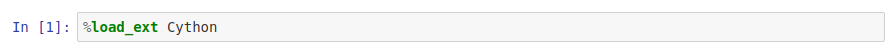
\includegraphics[width=0.98\paperwidth]{images/header.png}
    }
    \makebox[\textwidth][c]{
        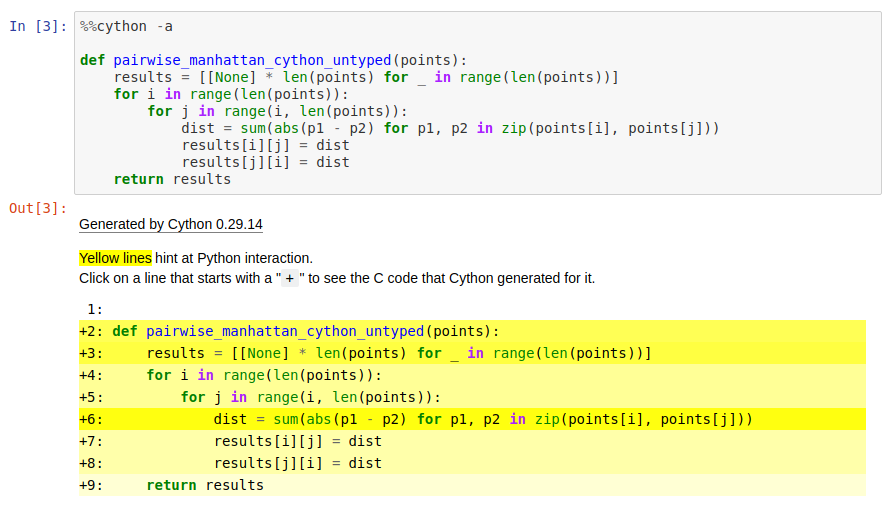
\includegraphics[width=0.98\paperwidth]{images/python-compiled.png}
    }
    \note{
        \begin{itemize}
            \item We use the \texttt{\%load\_ext Cython} magic so our notebook can compile Cython code
            \item Here we see the pure python implementation being compiled with Cython
            \item \texttt{\%\%cython -a} compiles the code in this cell and the \texttt{-a} adds annotation to the output
            \item The annotated view below tells us which lines (yellow) interact with the python interpretor
            \item General rule of thumb is yellow == slow
        \end{itemize}
    }
\end{frame}

\begin{frame}
    \makebox[\textwidth][c]{
        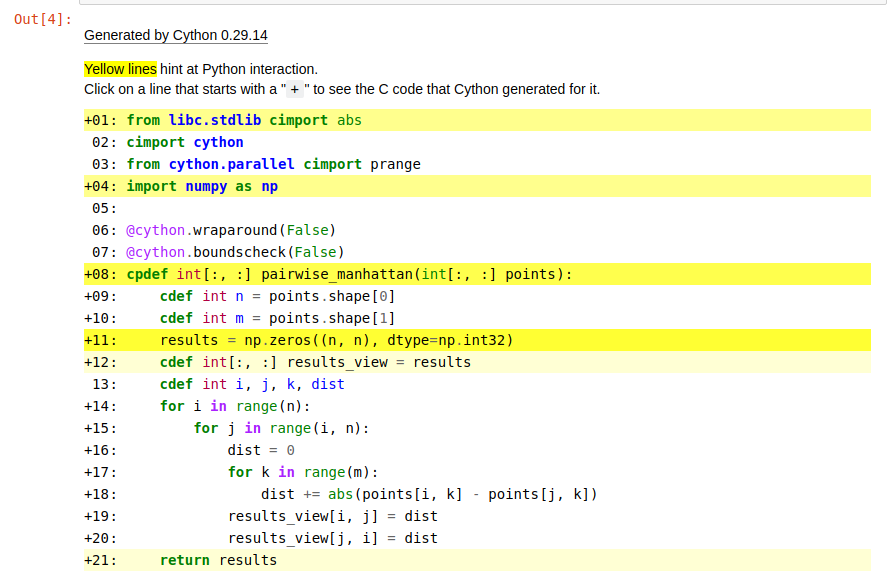
\includegraphics[width=0.98\paperwidth]{images/cython-annotation.png}
    }
    \note{
        \begin{itemize}
            \item This is the annotated version of the cython code
            \item We see some yellow, for example creating the \texttt{results} object but this is only dones once
            \item The whole actual calculation is all white, there is no python, only C
        \end{itemize}
    }
\end{frame}

\begin{frame}
    \makebox[\textwidth][c]{
        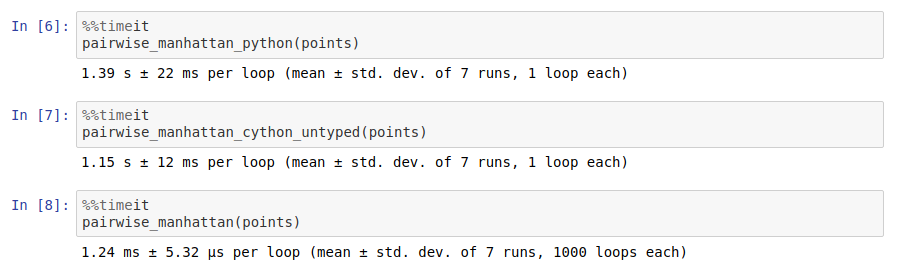
\includegraphics[width=0.98\paperwidth]{images/jupyter-speed.png}
    }
    \note{
        \begin{itemize}
            \item The compiled python version gives a slight boost
            \item The cython verions blows them out of the water
        \end{itemize}
    }
\end{frame}

\begin{section}{Conclusion}

\begin{frame}
    \frametitle{Conclusion}
    \begin{itemize}
        \item Vectorization and Broadcasting in NumPy lets us push loops from python into C
        \item Cython lets us write fast loops and is useful for speeding up difficult to vectorize code
        \item If you have a custom use case cython can often beat the more general NumPy solution
    \end{itemize}
    \note{
        \begin{itemize}
            \item As we saw in the numpy broadcasting it was a lot of extra work/complexity to remove the redundant computation which is easy in cython.
            \item As we saw in the numpy double broadcasting we can't remove the redundant computation.
        \end{itemize}
    }
\end{frame}

\begin{frame}
    \frametitle{Links}
    \begin{itemize}
        \item Notebook: \href{https://nbviewer.jupyter.org/github/blester125/MIPy-Talk-Jan-2-2020/blob/master/scripts/cython-jupyter-example.ipynb}{https://nbviewer.jupyter.org/github/blester125/MIPy-Talk-Jan-2-2020/blob/master/scripts/cython-jupyter-example.ipynb}
        \item Slides: \href{https://github.com/blester125/MIPy-Talk-Jan-2-2020/blob/master/slides/slides.pdf}{https://github.com/blester125/MIPy-Talk-Jan-2-2020/blob/master/slides/slides.pdf}
        \item Twitter: \href{https://twitter.com/BrianLester125}{https://twitter.com/BrianLester125}
        \item GitHub: \href{https://github.com/blester125}{https://github.com/blester125}
    \end{itemize}
    \note{
        \begin{itemize}
            \item The link to the slides is in a GitHub repo that has all these implementations, code to reproduce the graphs, and a docker container that has optimized versions of NumPy installed.
        \end{itemize}
    }
\end{frame}

\end{section} %Conclusion

\end{document}
